%% bm.pdf preamble - material merged from previous preamble and current pandoc preamable output
% NOTE: float placement required changes to the source files referenced by bm.tex
% May 28, 2020
%
% Use lualatex to compile - test with MiKTeX 2.9

% uncomment to list all files in log
%\listfiles

\documentclass[12pt]{report}


\usepackage{fontspec}

%\setmainfont[Scale=MatchLowercase]{Lucida Bright}
%\setmonofont{FreeMono}
%\setmonofont{Source Code Pro}
\setmonofont[Scale=MatchLowercase]{Ubuntu Mono}

% short snippets of asian languages
\newfontfamily\myAsian{Noto Serif TC Medium}

\usepackage[headings]{fullpage}

% national use characters 
%\usepackage{inputenc}

% ams mathematical symbols
\usepackage{amsmath,amssymb}

% added to support pandoc highlighting
\usepackage{microtype}

\usepackage{makeidx}

% add index and bibliographies to table of contents
\usepackage[nottoc]{tocbibind}

% postscript courier and times in place of cm fonts
%\usepackage{courier}
%\usepackage{times}

% extended coloring
\usepackage{color}
\usepackage[table,dvipsnames]{xcolor}
\usepackage{colortbl}

% advanced date formating
\usepackage{datetime}

%support pandoc code highlighting
\usepackage{fancyvrb}

% \DefineShortVerb[commandchars=\\\{\}]{\|}
% \DefineVerbatimEnvironment{Highlighting}{Verbatim}{commandchars=\\\{\}}
% % Add ',fontsize=\small' for more characters per line

% tango style colors
% \usepackage{framed}
% \definecolor{shadecolor}{RGB}{255,255,255}
% \newenvironment{Shaded}{\begin{snugshade}}{\end{snugshade}}
% \newcommand{\KeywordTok}[1]{\textcolor[rgb]{0.13,0.29,0.53}{\textbf{{#1}}}}
% \newcommand{\DataTypeTok}[1]{\textcolor[rgb]{0.13,0.29,0.53}{{#1}}}
% \newcommand{\DecValTok}[1]{\textcolor[rgb]{0.00,0.00,0.81}{{#1}}}
% \newcommand{\BaseNTok}[1]{\textcolor[rgb]{0.00,0.00,0.81}{{#1}}}
% \newcommand{\FloatTok}[1]{\textcolor[rgb]{0.00,0.00,0.81}{{#1}}}
% \newcommand{\CharTok}[1]{\textcolor[rgb]{0.31,0.60,0.02}{{#1}}}
% \newcommand{\StringTok}[1]{\textcolor[rgb]{0.31,0.60,0.02}{{#1}}}
% \newcommand{\CommentTok}[1]{\textcolor[rgb]{0.56,0.35,0.01}{\textit{{#1}}}}
% \newcommand{\OtherTok}[1]{\textcolor[rgb]{0.56,0.35,0.01}{{#1}}}
% \newcommand{\AlertTok}[1]{\textcolor[rgb]{0.94,0.16,0.16}{{#1}}}
% \newcommand{\FunctionTok}[1]{\textcolor[rgb]{0.00,0.00,0.00}{{#1}}}
% \newcommand{\RegionMarkerTok}[1]{{#1}}
% \newcommand{\ErrorTok}[1]{\textbf{{#1}}}
% \newcommand{\NormalTok}[1]{{#1}}

% %espresso style colors
% \usepackage{framed}
% \definecolor{shadecolor}{RGB}{42,33,28}
% \newenvironment{Shaded}{\begin{snugshade}}{\end{snugshade}}
% \newcommand{\KeywordTok}[1]{\textcolor[rgb]{0.26,0.66,0.93}{\textbf{{#1}}}}
% \newcommand{\DataTypeTok}[1]{\textcolor[rgb]{0.74,0.68,0.62}{\underline{{#1}}}}
% \newcommand{\DecValTok}[1]{\textcolor[rgb]{0.27,0.67,0.26}{{#1}}}
% \newcommand{\BaseNTok}[1]{\textcolor[rgb]{0.27,0.67,0.26}{{#1}}}
% \newcommand{\FloatTok}[1]{\textcolor[rgb]{0.27,0.67,0.26}{{#1}}}
% \newcommand{\CharTok}[1]{\textcolor[rgb]{0.02,0.61,0.04}{{#1}}}
% \newcommand{\StringTok}[1]{\textcolor[rgb]{0.02,0.61,0.04}{{#1}}}
% \newcommand{\CommentTok}[1]{\textcolor[rgb]{0.00,0.40,1.00}{\textit{{#1}}}}
% \newcommand{\OtherTok}[1]{\textcolor[rgb]{0.74,0.68,0.62}{{#1}}}
% \newcommand{\AlertTok}[1]{\textcolor[rgb]{1.00,1.00,0.00}{{#1}}}
% \newcommand{\FunctionTok}[1]{\textcolor[rgb]{1.00,0.58,0.35}{\textbf{{#1}}}}
% \newcommand{\RegionMarkerTok}[1]{\textcolor[rgb]{0.74,0.68,0.62}{{#1}}}
% \newcommand{\ErrorTok}[1]{\textcolor[rgb]{0.74,0.68,0.62}{\textbf{{#1}}}}
% \newcommand{\NormalTok}[1]{\textcolor[rgb]{0.74,0.68,0.62}{{#1}}}

% %kete style colors
% \newenvironment{Shaded}{}{}
% \newcommand{\KeywordTok}[1]{\textbf{{#1}}}
% \newcommand{\DataTypeTok}[1]{\textcolor[rgb]{0.50,0.00,0.00}{{#1}}}
% \newcommand{\DecValTok}[1]{\textcolor[rgb]{0.00,0.00,1.00}{{#1}}}
% \newcommand{\BaseNTok}[1]{\textcolor[rgb]{0.00,0.00,1.00}{{#1}}}
% \newcommand{\FloatTok}[1]{\textcolor[rgb]{0.50,0.00,0.50}{{#1}}}
% \newcommand{\CharTok}[1]{\textcolor[rgb]{1.00,0.00,1.00}{{#1}}}
% \newcommand{\StringTok}[1]{\textcolor[rgb]{0.87,0.00,0.00}{{#1}}}
% \newcommand{\CommentTok}[1]{\textcolor[rgb]{0.50,0.50,0.50}{\textit{{#1}}}}
% \newcommand{\OtherTok}[1]{{#1}}
% \newcommand{\AlertTok}[1]{\textcolor[rgb]{0.00,1.00,0.00}{\textbf{{#1}}}}
% \newcommand{\FunctionTok}[1]{\textcolor[rgb]{0.00,0.00,0.50}{{#1}}}
% \newcommand{\RegionMarkerTok}[1]{{#1}}
% \newcommand{\ErrorTok}[1]{\textcolor[rgb]{1.00,0.00,0.00}{\textbf{{#1}}}}
% \newcommand{\NormalTok}[1]{{#1}}
% %end pandoc code hacks

% jodliterate colors
\usepackage{color}
\definecolor{shadecolor}{RGB}{248,248,248}
% j control structures 
\definecolor{keywcolor}{rgb}{0.13,0.29,0.53}
% j explicit arguments x y m n u v
\definecolor{datacolor}{rgb}{0.13,0.29,0.53}
% j numbers - all types see j.xml
\definecolor{decvcolor}{rgb}{0.00,0.00,0.81}
\definecolor{basencolor}{rgb}{0.00,0.00,0.81}
\definecolor{floatcolor}{rgb}{0.00,0.00,0.81}
% j local assignments
\definecolor{charcolor}{rgb}{0.31,0.60,0.02}
\definecolor{stringcolor}{rgb}{0.31,0.60,0.02}
\definecolor{commentcolor}{rgb}{0.56,0.35,0.01}
% primitive adverbs and conjunctions
%\definecolor{othercolor}{rgb}{0.56,0.35,0.01}   
\definecolor{othercolor}{RGB}{0,0,255}
% global assignments
\definecolor{alertcolor}{rgb}{0.94,0.16,0.16}
% primitive J verbs and noun names
\definecolor{funccolor}{rgb}{0.00,0.00,0.00}

% custom colors
\definecolor{CodeBackGround}{cmyk}{0.0,0.0,0,0.05}    % light gray
\definecolor{CodeComment}{rgb}{0,0.50,0.00}           % dark green {0,0.45,0.08}
\definecolor{TableStripes}{gray}{0.9}                 % odd/even background in tables

% Colors for the hyperref package
\definecolor{urlcolor}{rgb}{0,.145,.698}
\definecolor{linkcolor}{rgb}{.71,0.21,0.01}
\definecolor{citecolor}{rgb}{.12,.54,.11}

% % Exact colors from NB
\definecolor{incolor}{HTML}{303F9F}
\definecolor{outcolor}{HTML}{D84315}
\definecolor{cellborder}{HTML}{CFCFCF}
\definecolor{cellbackground}{HTML}{F7F7F7}

% % ANSI colors
\definecolor{ansi-black}{HTML}{3E424D}
\definecolor{ansi-black-intense}{HTML}{282C36}
\definecolor{ansi-red}{HTML}{E75C58}
\definecolor{ansi-red-intense}{HTML}{B22B31}
\definecolor{ansi-green}{HTML}{00A250}
\definecolor{ansi-green-intense}{HTML}{007427}
\definecolor{ansi-yellow}{HTML}{DDB62B}
\definecolor{ansi-yellow-intense}{HTML}{B27D12}
\definecolor{ansi-blue}{HTML}{208FFB}
\definecolor{ansi-blue-intense}{HTML}{0065CA}
\definecolor{ansi-magenta}{HTML}{D160C4}
\definecolor{ansi-magenta-intense}{HTML}{A03196}
\definecolor{ansi-cyan}{HTML}{60C6C8}
\definecolor{ansi-cyan-intense}{HTML}{258F8F}
\definecolor{ansi-white}{HTML}{C5C1B4}
\definecolor{ansi-white-intense}{HTML}{A1A6B2}
\definecolor{ansi-default-inverse-fg}{HTML}{FFFFFF}
\definecolor{ansi-default-inverse-bg}{HTML}{000000}
    

% \usepackage{framed}
% \newenvironment{Shaded}{}{}
% \newcommand{\KeywordTok}[1]{\textcolor{keywcolor}{\textbf{{#1}}}}
% \newcommand{\DataTypeTok}[1]{\textcolor{datacolor}{{#1}}}
% %\newcommand{\DecValTok}[1]{\textcolor{decvcolor}{{#1}}}
% \newcommand{\DecValTok}[1]{{#1}} 
% \newcommand{\BaseNTok}[1]{\textcolor{basencolor}{{#1}}}
% \newcommand{\FloatTok}[1]{\textcolor{floatcolor}{{#1}}}
% \newcommand{\CharTok}[1]{\textcolor{charcolor}{\textbf{{#1}}}}
% \newcommand{\StringTok}[1]{\textcolor{stringcolor}{{#1}}}
% \newcommand{\CommentTok}[1]{\textcolor{commentcolor}{\textit{{#1}}}}
% \newcommand{\OtherTok}[1]{\textcolor{othercolor}{{#1}}} 
% \newcommand{\AlertTok}[1]{\textcolor{alertcolor}{\textbf{{#1}}}}
% %\newcommand{\FunctionTok}[1]{\textcolor{funccolor}{{#1}}}
% \newcommand{\FunctionTok}[1]{{#1}}
% \newcommand{\RegionMarkerTok}[1]{{#1}}
% \newcommand{\ErrorTok}[1]{\textbf{{#1}}}
% \newcommand{\NormalTok}[1]{{#1}}

% The default LaTeX title has an obnoxious amount of whitespace. By default,
% titling removes some of it. It also provides customization options.
\usepackage{titling}

% headers and footers
\usepackage{fancyhdr}
%\pagestyle{fancy}
\pagestyle{plain}

\fancyhead{}
\fancyfoot{}

%\fancyhead[LE,RO]{\slshape \rightmark}
%\fancyhead[LO,RE]{\slshape \leftmark}
\fancyfoot[C]{\thepage}
%\headrulewidth 0.4pt
%\footrulewidth 0 pt

%\addtolength{\headheight}{\baselineskip}

%\lfoot{\emph{Analyze the Data not the Drivel}}
%\rfoot{\emph{\today}}

% subfigure handles figures that contain subfigures
%\usepackage{color,graphicx,subfigure,sidecap}
\usepackage{graphicx,sidecap}
\usepackage{subfigure}
\graphicspath{{./inclusions/}}

% floatflt provides for text wrapping around small figures and tables
\usepackage{floatflt}

% tweak caption formats 
\usepackage{caption} 
\usepackage{sidecap}
%\usepackage{subcaption} % not compatible with subfigure

\usepackage{rotating} % flip tables sideways

% complex footnotes
%\usepackage{bigfoot}

% weird logos \XeLaTeX
\usepackage{metalogo}

\newcommand{\HRule}{\rule{\linewidth}{0.5mm}}

\usepackage[breakable]{tcolorbox}

\usepackage{parskip} % Stop auto-indenting (to mimic markdown behaviour)
    
% Basic figure setup, for now with no caption control since it's done
% automatically by Pandoc (which extracts ![](path) syntax from Markdown).
\usepackage{graphicx}

%\DeclareCaptionFormat{nocaption}{}
%\captionsetup{format=nocaption,aboveskip=0pt,belowskip=0pt}

\usepackage[Export]{adjustbox} % Used to constrain images to a maximum size
\adjustboxset{max size={0.9\linewidth}{0.9\paperheight}}
\usepackage{float}

%\floatplacement{figure}{H} % forces figures to be placed at the correct location

\usepackage{xcolor} % Allow colors to be defined
\usepackage{enumerate} % Needed for markdown enumerations to work
\usepackage{geometry} % Used to adjust the document margins

%\usepackage{amsmath} % Equations
%\usepackage{amssymb} % Equations

\usepackage{textcomp} % defines textquotesingle

% Hack from http://tex.stackexchange.com/a/47451/13684:
\AtBeginDocument{%
	\def\PYZsq{\textquotesingle}% Upright quotes in Pygmentized code
}

\usepackage{upquote} % Upright quotes for verbatim code
\usepackage{eurosym} % defines \euro
\usepackage[mathletters]{ucs} % Extended unicode (utf-8) support

%\usepackage{fancyvrb} % verbatim replacement that allows latex

\usepackage{grffile} % extends the file name processing of package graphics 
					 % to support a larger range
					 
\makeatletter % fix for grffile with XeLaTeX
\def\Gread@@xetex#1{%
  \IfFileExists{"\Gin@base".bb}%
  {\Gread@eps{\Gin@base.bb}}%
  {\Gread@@xetex@aux#1}%
}
\makeatother

% The hyperref package gives us a pdf with properly built
% internal navigation ('pdf bookmarks' for the table of contents,
% internal cross-reference links, web links for URLs, etc.)
\usepackage{hyperref}
% The default LaTeX title has an obnoxious amount of whitespace. By default,
% titling removes some of it. It also provides customization options.
\usepackage{titling}
\usepackage{longtable} % longtable support required by pandoc >1.10
\usepackage{booktabs}  % table support for pandoc > 1.12.2
\usepackage[inline]{enumitem} % IRkernel/repr support (it uses the enumerate* environment)
\usepackage[normalem]{ulem} % ulem is needed to support strikethroughs (\sout)
							% normalem makes italics be italics, not underlines
\usepackage{mathrsfs}

% commands and environments needed by pandoc snippets
% extracted from the output of `pandoc -s`
\providecommand{\tightlist}{%
  \setlength{\itemsep}{0pt}\setlength{\parskip}{0pt}}
  
\DefineVerbatimEnvironment{Highlighting}{Verbatim}{commandchars=\\\{\}}
% Add ',fontsize=\small' for more characters per line
\newenvironment{Shaded}{}{}
\newcommand{\KeywordTok}[1]{\textcolor[rgb]{0.00,0.44,0.13}{\textbf{{#1}}}}
\newcommand{\DataTypeTok}[1]{\textcolor[rgb]{0.56,0.13,0.00}{{#1}}}
\newcommand{\DecValTok}[1]{\textcolor[rgb]{0.25,0.63,0.44}{{#1}}}
\newcommand{\BaseNTok}[1]{\textcolor[rgb]{0.25,0.63,0.44}{{#1}}}
\newcommand{\FloatTok}[1]{\textcolor[rgb]{0.25,0.63,0.44}{{#1}}}
\newcommand{\CharTok}[1]{\textcolor[rgb]{0.25,0.44,0.63}{{#1}}}
\newcommand{\StringTok}[1]{\textcolor[rgb]{0.25,0.44,0.63}{{#1}}}
\newcommand{\CommentTok}[1]{\textcolor[rgb]{0.38,0.63,0.69}{\textit{{#1}}}}
\newcommand{\OtherTok}[1]{\textcolor[rgb]{0.00,0.44,0.13}{{#1}}}
\newcommand{\AlertTok}[1]{\textcolor[rgb]{1.00,0.00,0.00}{\textbf{{#1}}}}
\newcommand{\FunctionTok}[1]{\textcolor[rgb]{0.02,0.16,0.49}{{#1}}}
\newcommand{\RegionMarkerTok}[1]{{#1}}
\newcommand{\ErrorTok}[1]{\textcolor[rgb]{1.00,0.00,0.00}{\textbf{{#1}}}}
\newcommand{\NormalTok}[1]{{#1}}

% Additional commands for more recent versions of Pandoc
\newcommand{\ConstantTok}[1]{\textcolor[rgb]{0.53,0.00,0.00}{{#1}}}
\newcommand{\SpecialCharTok}[1]{\textcolor[rgb]{0.25,0.44,0.63}{{#1}}}
\newcommand{\VerbatimStringTok}[1]{\textcolor[rgb]{0.25,0.44,0.63}{{#1}}}
\newcommand{\SpecialStringTok}[1]{\textcolor[rgb]{0.73,0.40,0.53}{{#1}}}
\newcommand{\ImportTok}[1]{{#1}}
\newcommand{\DocumentationTok}[1]{\textcolor[rgb]{0.73,0.13,0.13}{\textit{{#1}}}}
\newcommand{\AnnotationTok}[1]{\textcolor[rgb]{0.38,0.63,0.69}{\textbf{\textit{{#1}}}}}
\newcommand{\CommentVarTok}[1]{\textcolor[rgb]{0.38,0.63,0.69}{\textbf{\textit{{#1}}}}}
\newcommand{\VariableTok}[1]{\textcolor[rgb]{0.10,0.09,0.49}{{#1}}}
\newcommand{\ControlFlowTok}[1]{\textcolor[rgb]{0.00,0.44,0.13}{\textbf{{#1}}}}
\newcommand{\OperatorTok}[1]{\textcolor[rgb]{0.40,0.40,0.40}{{#1}}}
\newcommand{\BuiltInTok}[1]{{#1}}
\newcommand{\ExtensionTok}[1]{{#1}}
\newcommand{\PreprocessorTok}[1]{\textcolor[rgb]{0.74,0.48,0.00}{{#1}}}
\newcommand{\AttributeTok}[1]{\textcolor[rgb]{0.49,0.56,0.16}{{#1}}}
\newcommand{\InformationTok}[1]{\textcolor[rgb]{0.38,0.63,0.69}{\textbf{\textit{{#1}}}}}
\newcommand{\WarningTok}[1]{\textcolor[rgb]{0.38,0.63,0.69}{\textbf{\textit{{#1}}}}}

% Define a nice break command that doesn't care if a line doesn't already exist.
\def\br{\hspace*{\fill} \\* }
% Math Jax compatibility definitions
\def\gt{>}
\def\lt{<}
\let\Oldtex\TeX
\let\Oldlatex\LaTeX
\renewcommand{\TeX}{\textrm{\Oldtex}}
\renewcommand{\LaTeX}{\textrm{\Oldlatex}}
 
% Pygments definitions
\makeatletter
\def\PY@reset{\let\PY@it=\relax \let\PY@bf=\relax%
    \let\PY@ul=\relax \let\PY@tc=\relax%
    \let\PY@bc=\relax \let\PY@ff=\relax}
\def\PY@tok#1{\csname PY@tok@#1\endcsname}
\def\PY@toks#1+{\ifx\relax#1\empty\else%
    \PY@tok{#1}\expandafter\PY@toks\fi}
\def\PY@do#1{\PY@bc{\PY@tc{\PY@ul{%
    \PY@it{\PY@bf{\PY@ff{#1}}}}}}}
\def\PY#1#2{\PY@reset\PY@toks#1+\relax+\PY@do{#2}}

\expandafter\def\csname PY@tok@w\endcsname{\def\PY@tc##1{\textcolor[rgb]{0.73,0.73,0.73}{##1}}}
\expandafter\def\csname PY@tok@c\endcsname{\let\PY@it=\textit\def\PY@tc##1{\textcolor[rgb]{0.25,0.50,0.50}{##1}}}
\expandafter\def\csname PY@tok@cp\endcsname{\def\PY@tc##1{\textcolor[rgb]{0.74,0.48,0.00}{##1}}}
\expandafter\def\csname PY@tok@k\endcsname{\let\PY@bf=\textbf\def\PY@tc##1{\textcolor[rgb]{0.00,0.50,0.00}{##1}}}
\expandafter\def\csname PY@tok@kp\endcsname{\def\PY@tc##1{\textcolor[rgb]{0.00,0.50,0.00}{##1}}}
\expandafter\def\csname PY@tok@kt\endcsname{\def\PY@tc##1{\textcolor[rgb]{0.69,0.00,0.25}{##1}}}
\expandafter\def\csname PY@tok@o\endcsname{\def\PY@tc##1{\textcolor[rgb]{0.40,0.40,0.40}{##1}}}
\expandafter\def\csname PY@tok@ow\endcsname{\let\PY@bf=\textbf\def\PY@tc##1{\textcolor[rgb]{0.67,0.13,1.00}{##1}}}
\expandafter\def\csname PY@tok@nb\endcsname{\def\PY@tc##1{\textcolor[rgb]{0.00,0.50,0.00}{##1}}}
\expandafter\def\csname PY@tok@nf\endcsname{\def\PY@tc##1{\textcolor[rgb]{0.00,0.00,1.00}{##1}}}
\expandafter\def\csname PY@tok@nc\endcsname{\let\PY@bf=\textbf\def\PY@tc##1{\textcolor[rgb]{0.00,0.00,1.00}{##1}}}
\expandafter\def\csname PY@tok@nn\endcsname{\let\PY@bf=\textbf\def\PY@tc##1{\textcolor[rgb]{0.00,0.00,1.00}{##1}}}
\expandafter\def\csname PY@tok@ne\endcsname{\let\PY@bf=\textbf\def\PY@tc##1{\textcolor[rgb]{0.82,0.25,0.23}{##1}}}
\expandafter\def\csname PY@tok@nv\endcsname{\def\PY@tc##1{\textcolor[rgb]{0.10,0.09,0.49}{##1}}}
\expandafter\def\csname PY@tok@no\endcsname{\def\PY@tc##1{\textcolor[rgb]{0.53,0.00,0.00}{##1}}}
\expandafter\def\csname PY@tok@nl\endcsname{\def\PY@tc##1{\textcolor[rgb]{0.63,0.63,0.00}{##1}}}
\expandafter\def\csname PY@tok@ni\endcsname{\let\PY@bf=\textbf\def\PY@tc##1{\textcolor[rgb]{0.60,0.60,0.60}{##1}}}
\expandafter\def\csname PY@tok@na\endcsname{\def\PY@tc##1{\textcolor[rgb]{0.49,0.56,0.16}{##1}}}
\expandafter\def\csname PY@tok@nt\endcsname{\let\PY@bf=\textbf\def\PY@tc##1{\textcolor[rgb]{0.00,0.50,0.00}{##1}}}
\expandafter\def\csname PY@tok@nd\endcsname{\def\PY@tc##1{\textcolor[rgb]{0.67,0.13,1.00}{##1}}}
\expandafter\def\csname PY@tok@s\endcsname{\def\PY@tc##1{\textcolor[rgb]{0.73,0.13,0.13}{##1}}}
\expandafter\def\csname PY@tok@sd\endcsname{\let\PY@it=\textit\def\PY@tc##1{\textcolor[rgb]{0.73,0.13,0.13}{##1}}}
\expandafter\def\csname PY@tok@si\endcsname{\let\PY@bf=\textbf\def\PY@tc##1{\textcolor[rgb]{0.73,0.40,0.53}{##1}}}
\expandafter\def\csname PY@tok@se\endcsname{\let\PY@bf=\textbf\def\PY@tc##1{\textcolor[rgb]{0.73,0.40,0.13}{##1}}}
\expandafter\def\csname PY@tok@sr\endcsname{\def\PY@tc##1{\textcolor[rgb]{0.73,0.40,0.53}{##1}}}
\expandafter\def\csname PY@tok@ss\endcsname{\def\PY@tc##1{\textcolor[rgb]{0.10,0.09,0.49}{##1}}}
\expandafter\def\csname PY@tok@sx\endcsname{\def\PY@tc##1{\textcolor[rgb]{0.00,0.50,0.00}{##1}}}
\expandafter\def\csname PY@tok@m\endcsname{\def\PY@tc##1{\textcolor[rgb]{0.40,0.40,0.40}{##1}}}
\expandafter\def\csname PY@tok@gh\endcsname{\let\PY@bf=\textbf\def\PY@tc##1{\textcolor[rgb]{0.00,0.00,0.50}{##1}}}
\expandafter\def\csname PY@tok@gu\endcsname{\let\PY@bf=\textbf\def\PY@tc##1{\textcolor[rgb]{0.50,0.00,0.50}{##1}}}
\expandafter\def\csname PY@tok@gd\endcsname{\def\PY@tc##1{\textcolor[rgb]{0.63,0.00,0.00}{##1}}}
\expandafter\def\csname PY@tok@gi\endcsname{\def\PY@tc##1{\textcolor[rgb]{0.00,0.63,0.00}{##1}}}
\expandafter\def\csname PY@tok@gr\endcsname{\def\PY@tc##1{\textcolor[rgb]{1.00,0.00,0.00}{##1}}}
\expandafter\def\csname PY@tok@ge\endcsname{\let\PY@it=\textit}
\expandafter\def\csname PY@tok@gs\endcsname{\let\PY@bf=\textbf}
\expandafter\def\csname PY@tok@gp\endcsname{\let\PY@bf=\textbf\def\PY@tc##1{\textcolor[rgb]{0.00,0.00,0.50}{##1}}}
\expandafter\def\csname PY@tok@go\endcsname{\def\PY@tc##1{\textcolor[rgb]{0.53,0.53,0.53}{##1}}}
\expandafter\def\csname PY@tok@gt\endcsname{\def\PY@tc##1{\textcolor[rgb]{0.00,0.27,0.87}{##1}}}
\expandafter\def\csname PY@tok@err\endcsname{\def\PY@bc##1{\setlength{\fboxsep}{0pt}\fcolorbox[rgb]{1.00,0.00,0.00}{1,1,1}{\strut ##1}}}
\expandafter\def\csname PY@tok@kc\endcsname{\let\PY@bf=\textbf\def\PY@tc##1{\textcolor[rgb]{0.00,0.50,0.00}{##1}}}
\expandafter\def\csname PY@tok@kd\endcsname{\let\PY@bf=\textbf\def\PY@tc##1{\textcolor[rgb]{0.00,0.50,0.00}{##1}}}
\expandafter\def\csname PY@tok@kn\endcsname{\let\PY@bf=\textbf\def\PY@tc##1{\textcolor[rgb]{0.00,0.50,0.00}{##1}}}
\expandafter\def\csname PY@tok@kr\endcsname{\let\PY@bf=\textbf\def\PY@tc##1{\textcolor[rgb]{0.00,0.50,0.00}{##1}}}
\expandafter\def\csname PY@tok@bp\endcsname{\def\PY@tc##1{\textcolor[rgb]{0.00,0.50,0.00}{##1}}}
\expandafter\def\csname PY@tok@fm\endcsname{\def\PY@tc##1{\textcolor[rgb]{0.00,0.00,1.00}{##1}}}
\expandafter\def\csname PY@tok@vc\endcsname{\def\PY@tc##1{\textcolor[rgb]{0.10,0.09,0.49}{##1}}}
\expandafter\def\csname PY@tok@vg\endcsname{\def\PY@tc##1{\textcolor[rgb]{0.10,0.09,0.49}{##1}}}
\expandafter\def\csname PY@tok@vi\endcsname{\def\PY@tc##1{\textcolor[rgb]{0.10,0.09,0.49}{##1}}}
\expandafter\def\csname PY@tok@vm\endcsname{\def\PY@tc##1{\textcolor[rgb]{0.10,0.09,0.49}{##1}}}
\expandafter\def\csname PY@tok@sa\endcsname{\def\PY@tc##1{\textcolor[rgb]{0.73,0.13,0.13}{##1}}}
\expandafter\def\csname PY@tok@sb\endcsname{\def\PY@tc##1{\textcolor[rgb]{0.73,0.13,0.13}{##1}}}
\expandafter\def\csname PY@tok@sc\endcsname{\def\PY@tc##1{\textcolor[rgb]{0.73,0.13,0.13}{##1}}}
\expandafter\def\csname PY@tok@dl\endcsname{\def\PY@tc##1{\textcolor[rgb]{0.73,0.13,0.13}{##1}}}
\expandafter\def\csname PY@tok@s2\endcsname{\def\PY@tc##1{\textcolor[rgb]{0.73,0.13,0.13}{##1}}}
\expandafter\def\csname PY@tok@sh\endcsname{\def\PY@tc##1{\textcolor[rgb]{0.73,0.13,0.13}{##1}}}
\expandafter\def\csname PY@tok@s1\endcsname{\def\PY@tc##1{\textcolor[rgb]{0.73,0.13,0.13}{##1}}}
\expandafter\def\csname PY@tok@mb\endcsname{\def\PY@tc##1{\textcolor[rgb]{0.40,0.40,0.40}{##1}}}
\expandafter\def\csname PY@tok@mf\endcsname{\def\PY@tc##1{\textcolor[rgb]{0.40,0.40,0.40}{##1}}}
\expandafter\def\csname PY@tok@mh\endcsname{\def\PY@tc##1{\textcolor[rgb]{0.40,0.40,0.40}{##1}}}
\expandafter\def\csname PY@tok@mi\endcsname{\def\PY@tc##1{\textcolor[rgb]{0.40,0.40,0.40}{##1}}}
\expandafter\def\csname PY@tok@il\endcsname{\def\PY@tc##1{\textcolor[rgb]{0.40,0.40,0.40}{##1}}}
\expandafter\def\csname PY@tok@mo\endcsname{\def\PY@tc##1{\textcolor[rgb]{0.40,0.40,0.40}{##1}}}
\expandafter\def\csname PY@tok@ch\endcsname{\let\PY@it=\textit\def\PY@tc##1{\textcolor[rgb]{0.25,0.50,0.50}{##1}}}
\expandafter\def\csname PY@tok@cm\endcsname{\let\PY@it=\textit\def\PY@tc##1{\textcolor[rgb]{0.25,0.50,0.50}{##1}}}
\expandafter\def\csname PY@tok@cpf\endcsname{\let\PY@it=\textit\def\PY@tc##1{\textcolor[rgb]{0.25,0.50,0.50}{##1}}}
\expandafter\def\csname PY@tok@c1\endcsname{\let\PY@it=\textit\def\PY@tc##1{\textcolor[rgb]{0.25,0.50,0.50}{##1}}}
\expandafter\def\csname PY@tok@cs\endcsname{\let\PY@it=\textit\def\PY@tc##1{\textcolor[rgb]{0.25,0.50,0.50}{##1}}}

\def\PYZbs{\char`\\}
\def\PYZus{\char`\_}
\def\PYZob{\char`\{}
\def\PYZcb{\char`\}}
\def\PYZca{\char`\^}
\def\PYZam{\char`\&}
\def\PYZlt{\char`\<}
\def\PYZgt{\char`\>}
\def\PYZsh{\char`\#}
\def\PYZpc{\char`\%}
\def\PYZdl{\char`\$}
\def\PYZhy{\char`\-}
\def\PYZsq{\char`\'}
\def\PYZdq{\char`\"}
\def\PYZti{\char`\~}
% for compatibility with earlier versions
\def\PYZat{@}
\def\PYZlb{[}
\def\PYZrb{]}
\makeatother

% For linebreaks inside Verbatim environment from package fancyvrb. 
\makeatletter
	\newbox\Wrappedcontinuationbox 
	\newbox\Wrappedvisiblespacebox 
	\newcommand*\Wrappedvisiblespace {\textcolor{red}{\textvisiblespace}} 
	\newcommand*\Wrappedcontinuationsymbol {\textcolor{red}{\llap{\tiny$\m@th\hookrightarrow$}}} 
	\newcommand*\Wrappedcontinuationindent {3ex } 
	\newcommand*\Wrappedafterbreak {\kern\Wrappedcontinuationindent\copy\Wrappedcontinuationbox} 
	% Take advantage of the already applied Pygments mark-up to insert 
	% potential linebreaks for TeX processing. 
	%        {, <, #, %, $, ' and ": go to next line. 
	%        _, }, ^, &, >, - and ~: stay at end of broken line. 
	% Use of \textquotesingle for straight quote. 
	\newcommand*\Wrappedbreaksatspecials {% 
		\def\PYGZus{\discretionary{\char`\_}{\Wrappedafterbreak}{\char`\_}}% 
		\def\PYGZob{\discretionary{}{\Wrappedafterbreak\char`\{}{\char`\{}}% 
		\def\PYGZcb{\discretionary{\char`\}}{\Wrappedafterbreak}{\char`\}}}% 
		\def\PYGZca{\discretionary{\char`\^}{\Wrappedafterbreak}{\char`\^}}% 
		\def\PYGZam{\discretionary{\char`\&}{\Wrappedafterbreak}{\char`\&}}% 
		\def\PYGZlt{\discretionary{}{\Wrappedafterbreak\char`\<}{\char`\<}}% 
		\def\PYGZgt{\discretionary{\char`\>}{\Wrappedafterbreak}{\char`\>}}% 
		\def\PYGZsh{\discretionary{}{\Wrappedafterbreak\char`\#}{\char`\#}}% 
		\def\PYGZpc{\discretionary{}{\Wrappedafterbreak\char`\%}{\char`\%}}% 
		\def\PYGZdl{\discretionary{}{\Wrappedafterbreak\char`\$}{\char`\$}}% 
		\def\PYGZhy{\discretionary{\char`\-}{\Wrappedafterbreak}{\char`\-}}% 
		\def\PYGZsq{\discretionary{}{\Wrappedafterbreak\textquotesingle}{\textquotesingle}}% 
		\def\PYGZdq{\discretionary{}{\Wrappedafterbreak\char`\"}{\char`\"}}% 
		\def\PYGZti{\discretionary{\char`\~}{\Wrappedafterbreak}{\char`\~}}% 
	} 
	% Some characters . , ; ? ! / are not pygmentized. 
	% This macro makes them "active" and they will insert potential linebreaks 
	\newcommand*\Wrappedbreaksatpunct {% 
		\lccode`\~`\.\lowercase{\def~}{\discretionary{\hbox{\char`\.}}{\Wrappedafterbreak}{\hbox{\char`\.}}}% 
		\lccode`\~`\,\lowercase{\def~}{\discretionary{\hbox{\char`\,}}{\Wrappedafterbreak}{\hbox{\char`\,}}}% 
		\lccode`\~`\;\lowercase{\def~}{\discretionary{\hbox{\char`\;}}{\Wrappedafterbreak}{\hbox{\char`\;}}}% 
		\lccode`\~`\:\lowercase{\def~}{\discretionary{\hbox{\char`\:}}{\Wrappedafterbreak}{\hbox{\char`\:}}}% 
		\lccode`\~`\?\lowercase{\def~}{\discretionary{\hbox{\char`\?}}{\Wrappedafterbreak}{\hbox{\char`\?}}}% 
		\lccode`\~`\!\lowercase{\def~}{\discretionary{\hbox{\char`\!}}{\Wrappedafterbreak}{\hbox{\char`\!}}}% 
		\lccode`\~`\/\lowercase{\def~}{\discretionary{\hbox{\char`\/}}{\Wrappedafterbreak}{\hbox{\char`\/}}}% 
		\catcode`\.\active
		\catcode`\,\active 
		\catcode`\;\active
		\catcode`\:\active
		\catcode`\?\active
		\catcode`\!\active
		\catcode`\/\active 
		\lccode`\~`\~ 	
	}
\makeatother

\let\OriginalVerbatim=\Verbatim
\makeatletter
\renewcommand{\Verbatim}[1][1]{%
	%\parskip\z@skip
	\sbox\Wrappedcontinuationbox {\Wrappedcontinuationsymbol}%
	\sbox\Wrappedvisiblespacebox {\FV@SetupFont\Wrappedvisiblespace}%
	\def\FancyVerbFormatLine ##1{\hsize\linewidth
		\vtop{\raggedright\hyphenpenalty\z@\exhyphenpenalty\z@
			\doublehyphendemerits\z@\finalhyphendemerits\z@
			\strut ##1\strut}%
	}%
	% If the linebreak is at a space, the latter will be displayed as visible
	% space at end of first line, and a continuation symbol starts next line.
	% Stretch/shrink are however usually zero for typewriter font.
	\def\FV@Space {%
		\nobreak\hskip\z@ plus\fontdimen3\font minus\fontdimen4\font
		\discretionary{\copy\Wrappedvisiblespacebox}{\Wrappedafterbreak}
		{\kern\fontdimen2\font}%
	}%
	
	% Allow breaks at special characters using \PYG... macros.
	\Wrappedbreaksatspecials
	% Breaks at punctuation characters . , ; ? ! and / need catcode=\active 	
	\OriginalVerbatim[#1,codes*=\Wrappedbreaksatpunct]%
}
\makeatother


% prompt
\makeatletter
\newcommand{\boxspacing}{\kern\kvtcb@left@rule\kern\kvtcb@boxsep}
\makeatother
\newcommand{\prompt}[4]{
	\ttfamily\llap{{\color{#2}[#3]:\hspace{3pt}#4}}\vspace{-\baselineskip}
}
    

% Prevent overflowing lines due to hard-to-break entities
\sloppy 

% Setup hyperref package
\hypersetup{
  breaklinks=true,  % so long urls are correctly broken across lines
  colorlinks=true,
  urlcolor=urlcolor,
  linkcolor=linkcolor,
  citecolor=citecolor,
  pdfauthor={John D. Baker},
  pdftitle={Analyze the Data not the Drivel},
  pdfsubject={Blog},
  pdfcreator={MikTeX+LaTeXe},
  pdfkeywords={blog,wordpress},
  }
  
% Slightly bigger margins than the latex defaults
% \geometry{verbose,tmargin=1in,bmargin=1in,lmargin=1in,rmargin=1in}  

%\usepackage{wrapfig}

% source code listings
\usepackage{listings}

\lstdefinelanguage{bat}
{morekeywords={echo,title,pushd,popd,setlocal,endlocal,off,if,not,exist,set,goto,pause},
sensitive=True,
morecomment=[l]{rem}
}

\lstdefinelanguage{jdoc}
{
morekeywords={},
otherkeywords={assert.,break.,continue.,for.,do.,if.,else.,elseif.,return.,select.,end.
,while.,whilst.,throw.,catch.,catchd.,catcht.,try.,case.,fcase.},
sensitive=True,
morecomment=[l]{NB.},
morestring=[b]',
morestring=[d]',
}

% latex size ordering - can never remember it
% \tiny
% \scriptsize
% \footnotesize
% \small
% \normalsize
% \large
% \Large
% \LARGE
% \huge
% \Huge
 
% listings package settings  
\lstset{%
  language=jdoc,                                % j document settings
  basicstyle=\ttfamily\footnotesize,            
  keywordstyle=\bfseries\color{keywcolor}\footnotesize,
  identifierstyle=\color{black},
  commentstyle=\slshape\color{CodeComment},     % colored slanted comments
  stringstyle=\color{red}\ttfamily,
  showstringspaces=false,                       
  %backgroundcolor=\color{CodeBackGround},       
  frame=single,                                
  framesep=1pt,                                 
  framerule=0.8pt,                             
  rulecolor=\color{CodeBackGround},   
  showspaces=false,
  %columns=fullflexible,
  %numbers=left,
  %numberstyle=\footnotesize,
  %numbersep=9pt,
  tabsize=2,
  showtabs=false,
  captionpos=b
  breaklines=true,                              
  breakindent=5pt                              
}

\lstdefinelanguage{JavaScript}{
  keywords={typeof, new, true, false, catch, function, return, null, catch, switch, var, if, in, while, do, else, case, break},
  ndkeywords={class, export, boolean, throw, implements, import, this},
  ndkeywordstyle=\color{darkgray}\bfseries,
  sensitive=false,
  comment=[l]{//},
  morecomment=[s]{/*}{*/},
  morestring=[b]',
  morestring=[b]"
}

% C# settings
\lstdefinestyle{sharpc}{
language=[Sharp]C,
basicstyle=\ttfamily\scriptsize, 
keywordstyle=\bfseries\color{keywcolor}\scriptsize,
framerule=0pt
}

% for source code listing longer than two use smaller font
\lstdefinestyle{smallersource}{
basicstyle=\ttfamily\scriptsize, 
keywordstyle=\bfseries\color{keywcolor}\scriptsize,
framerule=0pt
}

\lstdefinestyle{resetdefaults}{
language=jdoc,
basicstyle=\ttfamily\footnotesize,  
keywordstyle=\bfseries\color{keywcolor}\footnotesize,                                                               
framerule=0.8pt 
}

% APL UTF8 code points listed for lstlisting processing
\makeatletter
\lst@InputCatcodes
\def\lst@DefEC{%
 \lst@CCECUse \lst@ProcessLetter
  ^^80^^81^^82^^83^^84^^85^^86^^87^^88^^89^^8a^^8b^^8c^^8d^^8e^^8f%
  ^^90^^91^^92^^93^^94^^95^^96^^97^^98^^99^^9a^^9b^^9c^^9d^^9e^^9f%
  ^^a0^^a1^^a2^^a3^^a4^^a5^^a6^^a7^^a8^^a9^^aa^^ab^^ac^^ad^^ae^^af%
  ^^b0^^b1^^b2^^b3^^b4^^b5^^b6^^b7^^b8^^b9^^ba^^bb^^bc^^bd^^be^^bf%
  ^^c0^^c1^^c2^^c3^^c4^^c5^^c6^^c7^^c8^^c9^^ca^^cb^^cc^^cd^^ce^^cf%
  ^^d0^^d1^^d2^^d3^^d4^^d5^^d6^^d7^^d8^^d9^^da^^db^^dc^^dd^^de^^df%
  ^^e0^^e1^^e2^^e3^^e4^^e5^^e6^^e7^^e8^^e9^^ea^^eb^^ec^^ed^^ee^^ef%
  ^^f0^^f1^^f2^^f3^^f4^^f5^^f6^^f7^^f8^^f9^^fa^^fb^^fc^^fd^^fe^^ff%
  ^^^^20ac^^^^0153^^^^0152%
  ^^^^20a7^^^^2190^^^^2191^^^^2192^^^^2193^^^^2206^^^^2207^^^^220a%
  ^^^^2218^^^^2228^^^^2229^^^^222a^^^^2235^^^^223c^^^^2260^^^^2261%
  ^^^^2262^^^^2264^^^^2265^^^^2282^^^^2283^^^^2296^^^^22a2^^^^22a3%
  ^^^^22a4^^^^22a5^^^^22c4^^^^2308^^^^230a^^^^2336^^^^2337^^^^2339%
  ^^^^233b^^^^233d^^^^233f^^^^2340^^^^2342^^^^2347^^^^2348^^^^2349%
  ^^^^234b^^^^234e^^^^2350^^^^2352^^^^2355^^^^2357^^^^2359^^^^235d%
  ^^^^235e^^^^235f^^^^2361^^^^2362^^^^2363^^^^2364^^^^2365^^^^2368%
  ^^^^236a^^^^236b^^^^236c^^^^2371^^^^2372^^^^2373^^^^2374^^^^2375%
  ^^^^2377^^^^2378^^^^237a^^^^2395^^^^25af^^^^25ca^^^^25cb%  
  ^^00}
\lst@RestoreCatcodes
\makeatother

% custom lengths used within minipages
\newcommand{\minindent}{17pt}

\makeindex

\begin{document}

\subsection*{\href{http://analyzethedatanotthedrivel.org/2022/12/09/travel-diary-melbourne-and-uluru-part-2/}{Travel Diary: Melbourne and Uluru (Part 2)}}
\addcontentsline{toc}{subsection}{Travel Diary: Melbourne and Uluru (Part 2)}


\noindent\emph{Posted: 09 Dec 2022 20:55:41}
\vspace{6pt}

\emph{This is the second installment of my Australia New Zealand travel
notes}. \emph{Click on any of the images to jump to
\href{https://conceptcontrol.smugmug.com/Trips/Overseas/Australia-New-Zealand-2022/}{my
photo gallery} for this trip.}


\hypertarget{day-10-oct-17-2022}{%
\paragraph{\texorpdfstring{\textbf{Day 10 Oct 17, 
2022}}{Day 10 Oct 17, 2022}}\label{day-10-oct-17-2022}}

\textbf{Park Hyatt, Melbourne Victoria, iPhone}

This morning we had breakfast at the Mantra Albury Hotel and then did a
little bit of shopping. Mali had spotted a Katmandu store the previous
evening while we were looking for a place to eat. We ate in a Mediterranean 
restaurant that was staffed by Indians. Mali picked up a
shirt and hat at Katmandu while I had a flat white coffee in a nearby
cafe.

After Katmandu, we checked out the
\href{https://www.mamalbury.com.au/}{Murray Art Museum of Albury
(MAMA)}. It was a nice little museum with friendly staff. They were in
the middle of changing exhibits. The exhibit change was more interesting
than the art.

\captionsetup[figure]{labelformat=empty}
\begin{SCfigure}
\centering
\href{https://conceptcontrol.smugmug.com/Trips/Overseas/Australia-New-Zealand-2022/i-Z5hXNjd/A}{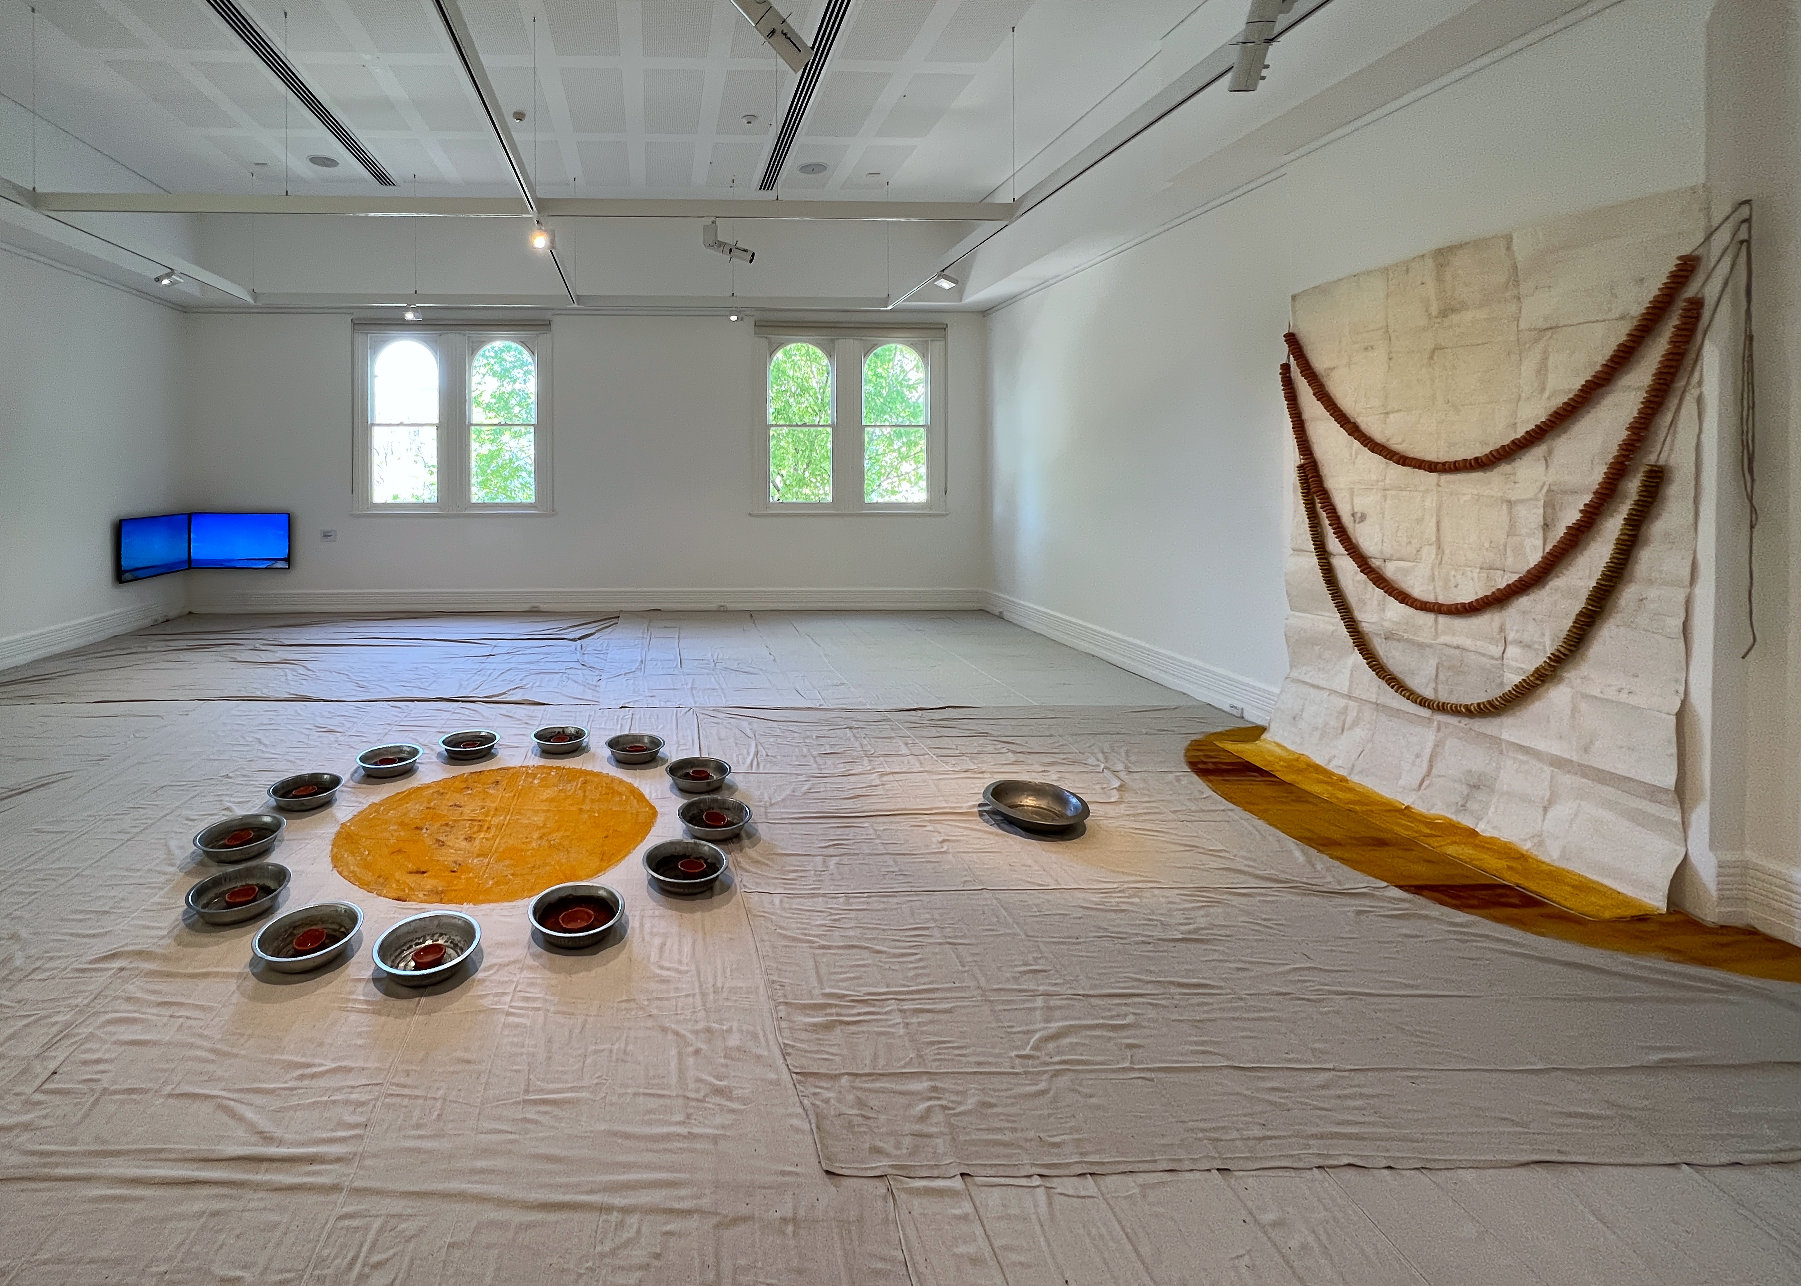
\includegraphics[width=0.40\textwidth]{mama-muesum-room-art.jpg}}
\caption[MAMA Art museum room]{Modern art takes odd forms. This mostly empty \href{https://www.mamalbury.com.au/}{MAMA museum} room
is a singular silly art piece.}
\label{fig:7573x0}
\end{SCfigure}

Then we drove from Albury toward Melbourne. Along the way, we turned
south on the Great Alpine Road and got as far as Bright Victoria. At
Bright, Mali found a natural clothing store, and we got hoodies. Our
Canadian credit cards were rejected but Mali's US card went through. We
brooded about the card refusal on the way to Melbourne.

In Melbourne, we checked in at the
\href{https://www.hyatt.com/en-US/hotel/australia/park-hyatt-melbourne/melph}{Park
Hyatt} and Mali's card was accepted without problems. Something was
probably wrong with the Bright store card reader but, just in case, we
VPN'ed into our Canadian bank and Mali paid off her Canadian VISA.

Tomorrow, we walk around Melbourne. They have free trams which will help
get around town.

\hypertarget{day-1112-oct-1819-2022}{%
\paragraph{\texorpdfstring{\textbf{Day 11,12 Oct 18,19 2022}}{Day 11,12 Oct 18,19 2022}}\label{day-1112-oct-1819-2022}}


\textbf{Ayers Rock Resort, NT, Mac}

On the 18\textsuperscript{th} we spent the day touring downtown
Melbourne. Melbourne has a free city core tram system. You can get on
the green and yellow trams in the free zone and ride around the city
without paying. It makes the entire core very accessible.


\captionsetup[figure]{labelformat=empty}
\begin{SCfigure}[10]
\centering
\href{https://conceptcontrol.smugmug.com/Trips/Overseas/Australia-New-Zealand-2022/i-gzRJZgc/A}{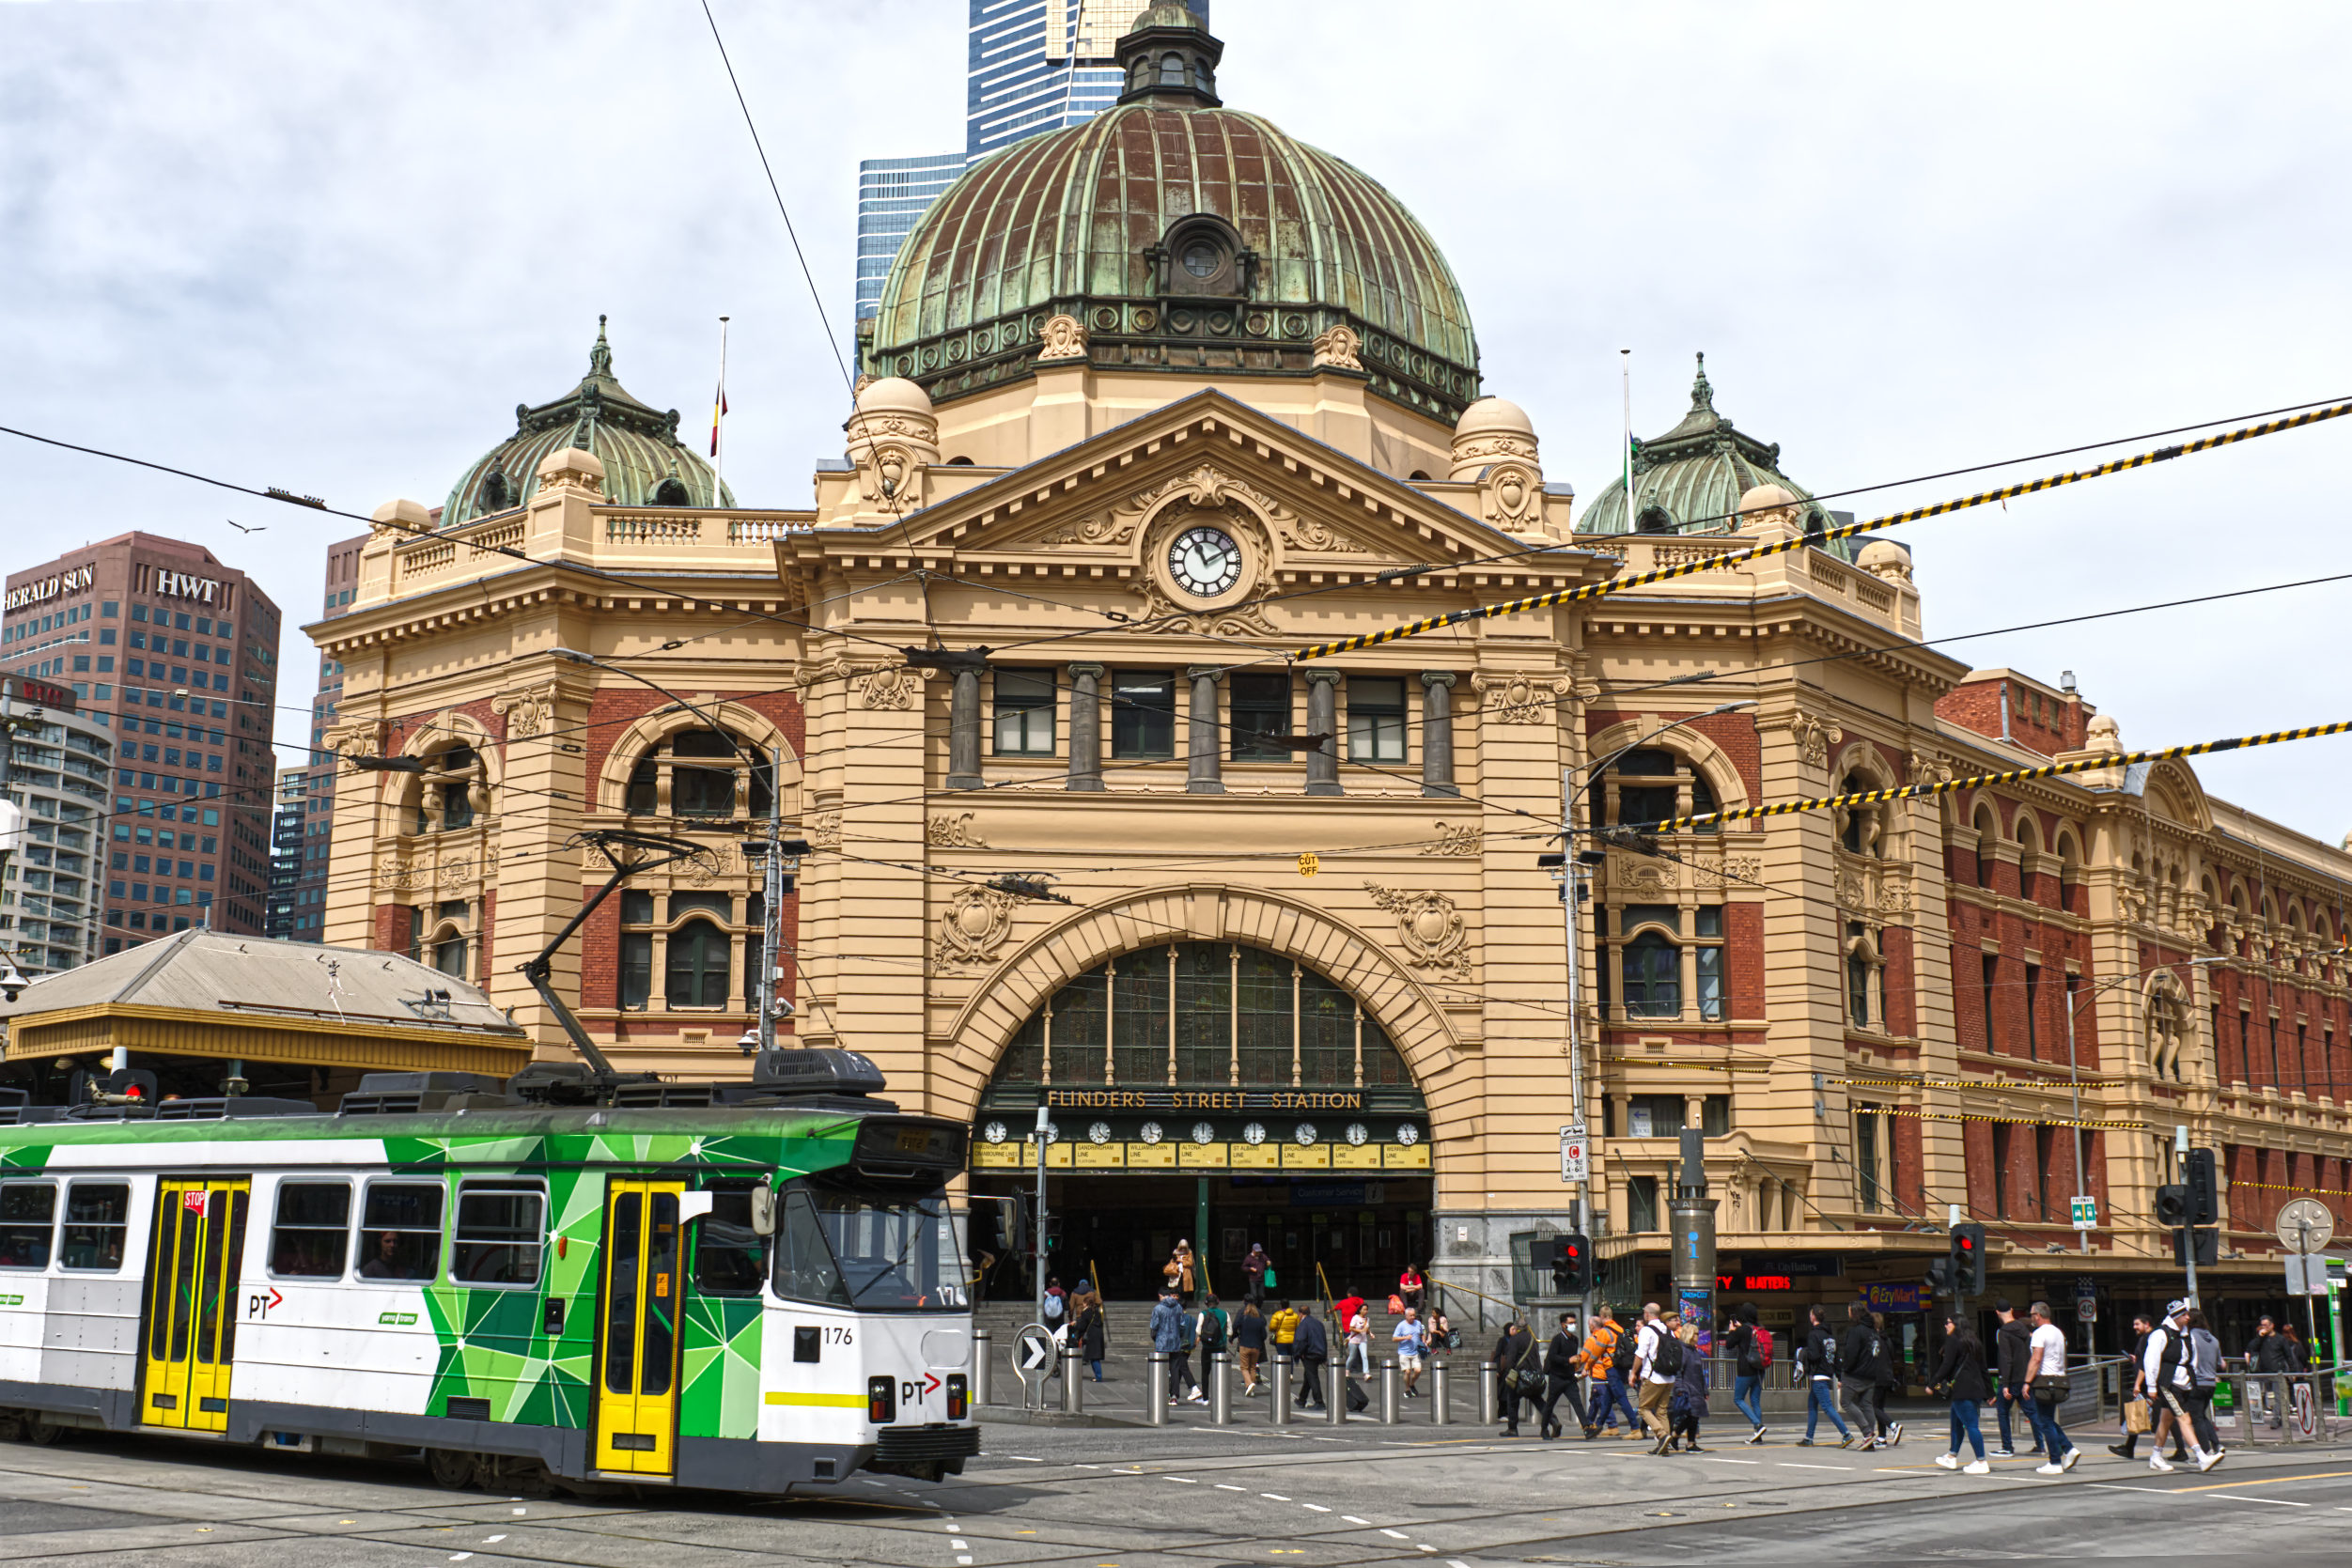
\includegraphics[width=0.40\textwidth]{flinders-street-station-melbourne.jpg}}
\caption[Flinders Street Station in Melbourne]{Flinders Street Station in Melbourne.}
\label{fig:7573x1}
\end{SCfigure}

We visited, The Royal Arcade, disappointing. It's an old shopping mall
dating from the 1870s. We ate breakfast at a cafe near the end of the
mall. We sat outside the cafe in the mall concourse; it was cold! Then
we walked across the street to The Block. Much nicer but still a mall. I
sat in a barber's chair outside the oldest barbershop in the world. It
was started in 1805. Then we rode the trolley up to Franklin Street.
Mali wanted to get an invoice for our car rental. After getting the
invoice we checked on The Victoria Market: a very large city market that
still functions as an actual market. Many such markets around the world
have degenerated into tourist traps. Mali picked up a dark brown
Kangaroo leather hat for me. The hat's big selling point: kangaroo
leather is lighter and tougher than normal leather.

After the market, we rode the tram back toward the river and got off at
Flinders Street, and then walked to the
\href{https://www.ngv.vic.gov.au/}{NGV Art Museum}. I looked through the
museum while Mali checked out the gift shop. Lots of school kids in
their neat school uniforms were visiting the museum. Many were sketching
in galleries. After NGV we checked out Melbourne's ``Freak Alley,''
called Hosier Lane. It's another alley filled with graffiti.
Surprisingly Boise's alley is much better.

After the alley, we headed across the river and stopped in at the Royal
Victoria Gallery. A very imposing building filled with more art than you
can see in a short visit. After this gallery, we popped across the
street and sat on a park bench beside the Edward VII statue. Then we
trammed back to La Trobe Street, changed trams, and visited the National
Exhibition Grounds and the Melbourne Museum. We finished the day by
having a steak dinner at the
\href{https://www.meatmaiden.com.au/}{Meatmaiden} followed by a
stressful refueling of the rental car for the next day's return. Why is
it that finding gas stations in major urban centers is such a fricking
pain?


\captionsetup[figure]{labelformat=empty}
\begin{figure}[htbp]
\centering
\href{https://conceptcontrol.smugmug.com/Trips/Overseas/Australia-New-Zealand-2022/i-LRj5GB9/A}{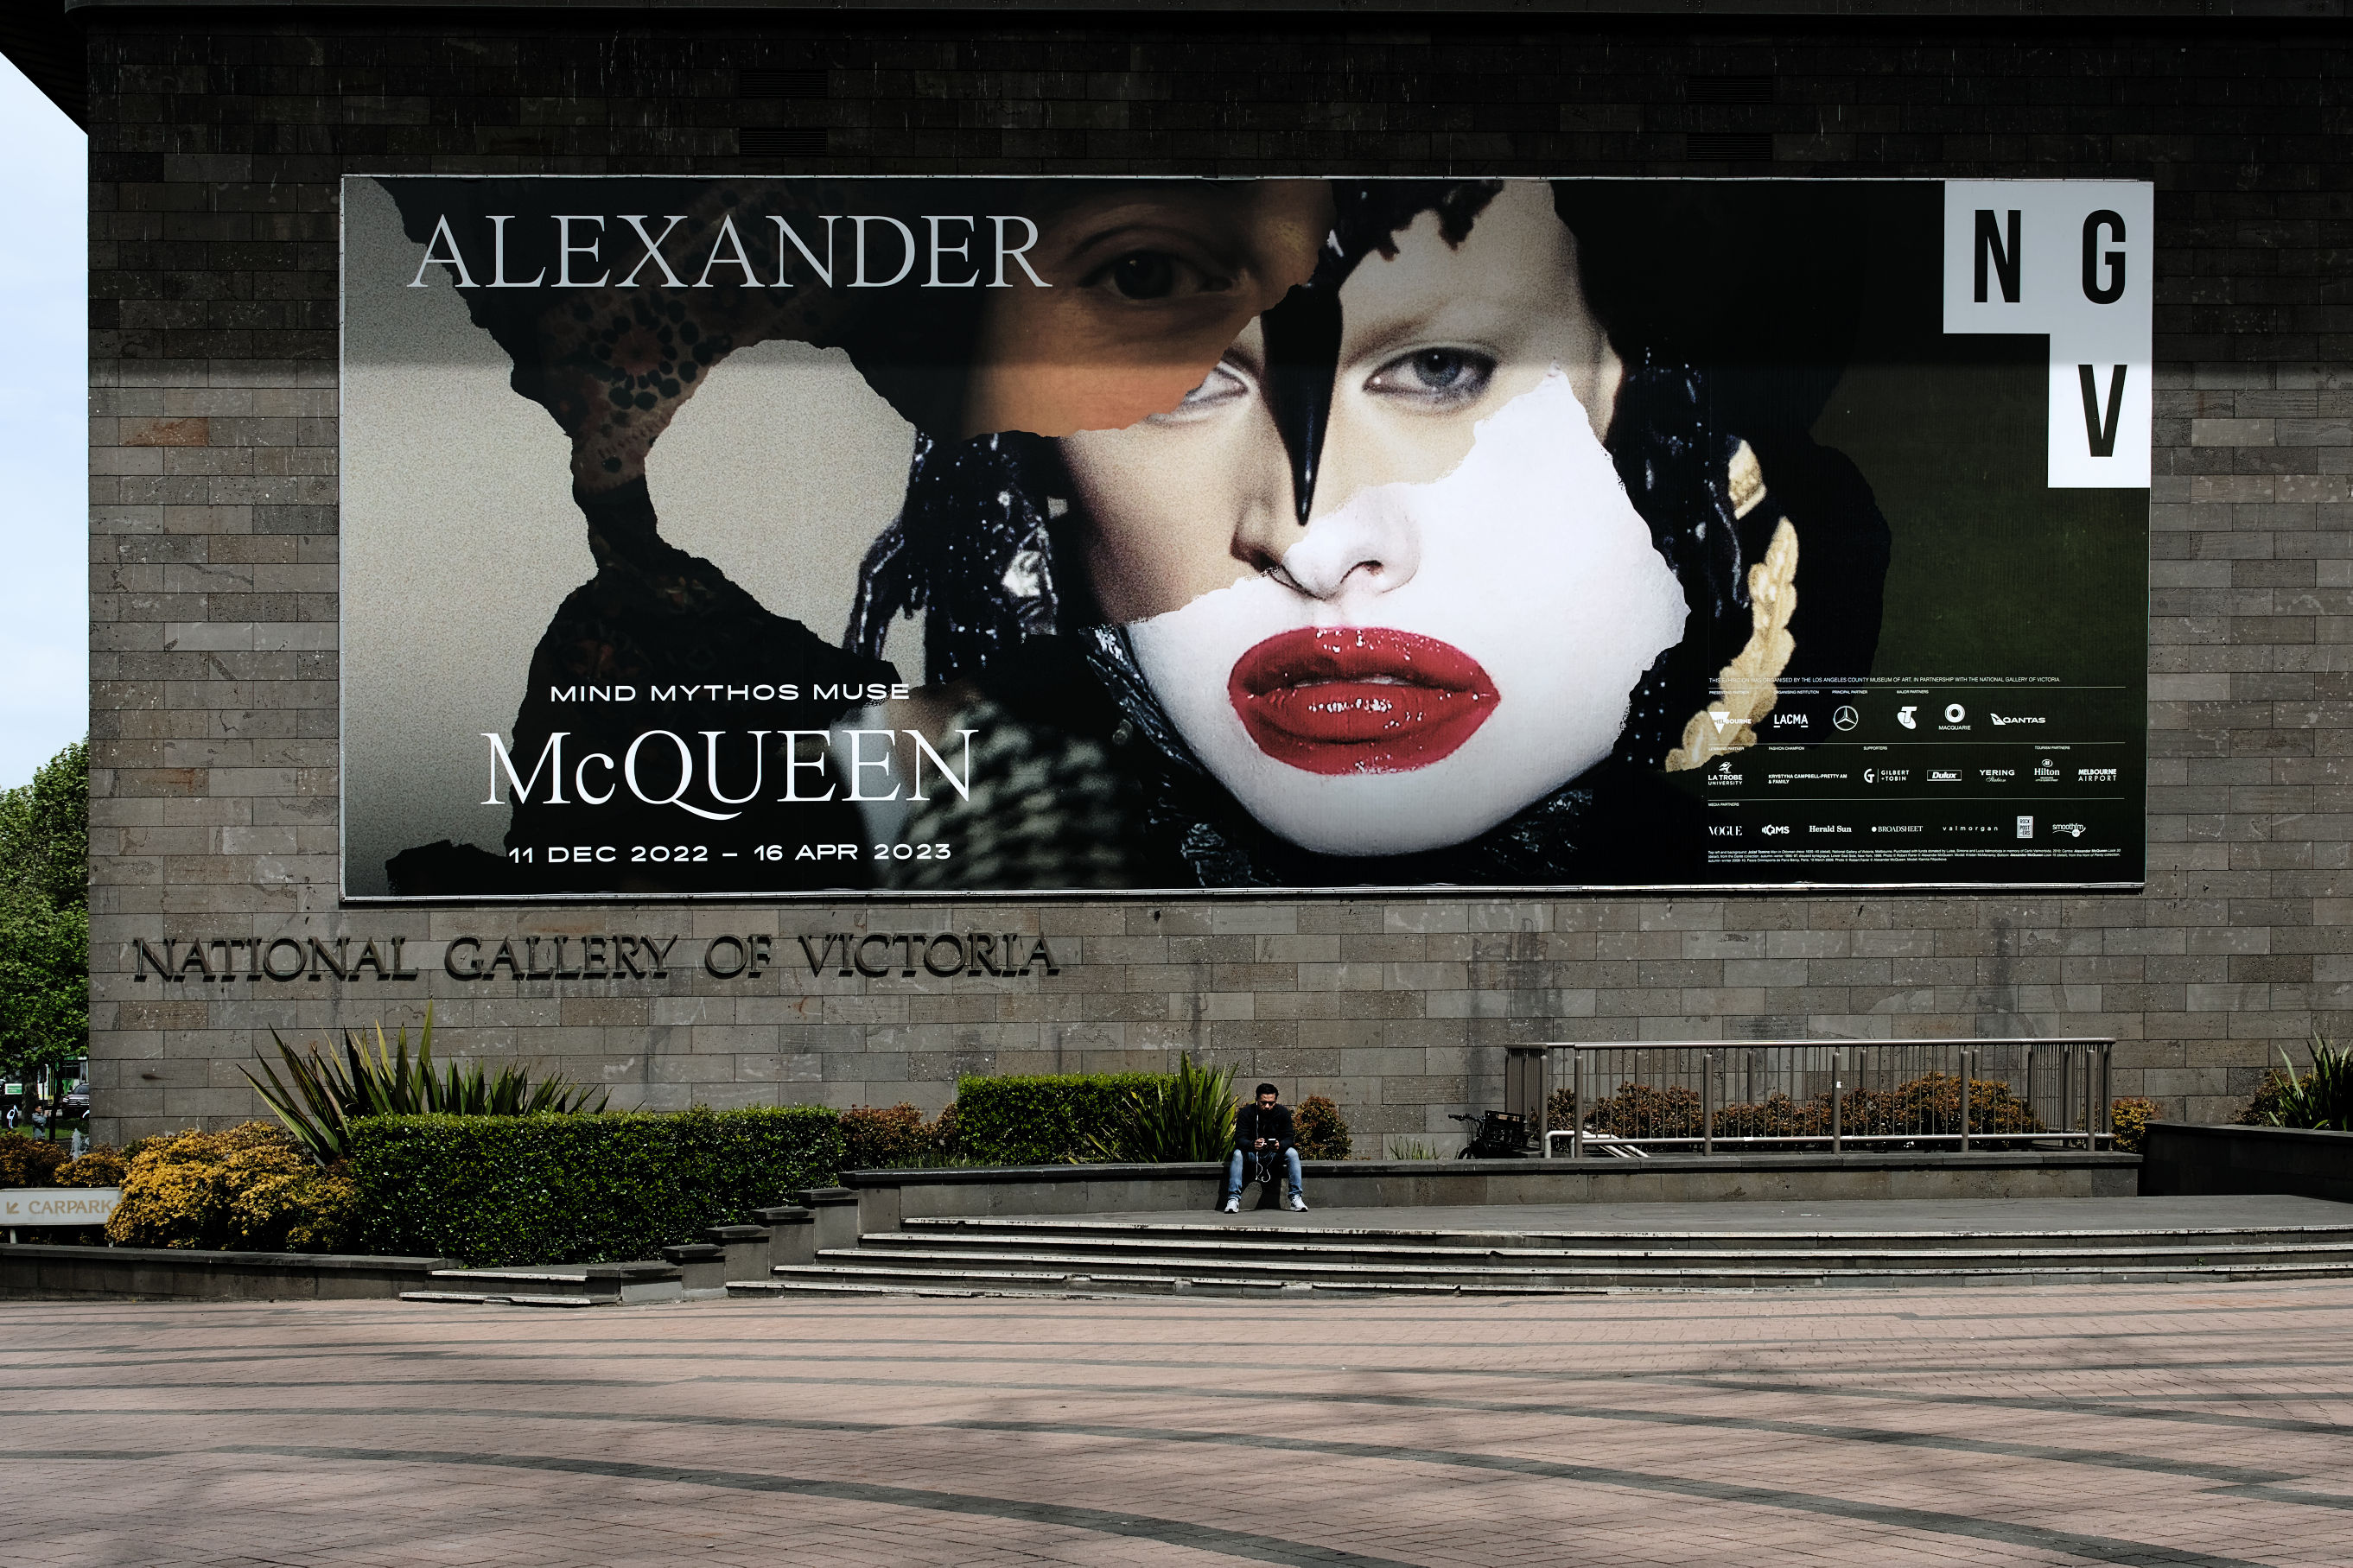
\includegraphics[width=0.50\textwidth]{national-gallery-victoria-sign.jpg}}
 \caption{National Gallery of Victoria.}
\label{fig:7573x2}
\end{figure}

Today, the 19\textsuperscript{th} we left the Park Hyatt, drove to the
Melbourne airport, and flew to Uluru. We got zinged for overweight
carry-ons. Two of our bags had to be checked. My computer with my two
backup drives was checked. On the return flight, I will transfer one USB
drive to my camera bags. It doesn't help to put all your redundant
storage devices in the same place. \emph{You're either backed up or
fucked up. Care to go over the options again?}

In half an hour, we will be going for an Uluru sunset and barbecue. I am
taking both my Nikons.

\emph{Later: the Uluru sunset lived up to the hype. We took pictures and
had champagne as the sun set but the barbecue after the sun went down
exceeded my expectations.} It was held right beside Uluru. After dinner,
our hosts turned off all lights and staged a star party. It was fabulous.
We saw the Magellanic Clouds, Alpha and Beta Centauri, Jupiter, Saturn,
and all of Scorpio: upside down. The Milky Way ran from horizon to
horizon with the central bulge, never completely seen in the northern
hemisphere, overhead. It was the best view of the galaxy I've ever had:
just awesome!

\hypertarget{day-1314-oct-2021-2022}{%
\paragraph{\texorpdfstring{\textbf{Day 13,14 Oct 20,21 2022}}{Day 13,14 Oct 20,21 2022}}\label{day-1314-oct-2021-2022}}

\textbf{Fullerton Hotel, Sydney NSW, Mac}

I am sitting at a rather nice desk in room 603 of the
\href{https://www.fullertonhotels.com/fullerton-hotel-sydney}{Fullerton
Hotel} in downtown Sydney with a double flat white coffee beside my Mac
as I write this. I will opine about Australia's superior coffee machines
someday but not now. This is a catch-up.

On Oct 20th I got up at 4:00 am to catch the ``Hop On Hop Off'' bus to
Kata Tjuta. I wanted to see both of the famous rock formations in the
national park but Mali didn't and decided she would rather sleep in. I'm
glad I got up. While waiting for the bus in the parking area of
\href{https://www.ayersrockresort.com.au/accommodation/desert-gardens-hotel}{The
Desert Gardens} I spotted Orion almost overhead and upside down. The
Orion Nebula was easily seen in my 8x42 Maven binoculars. The planet
Mars was also up: very orange, very bright. Once on the bus, we drove to
an observing platform about 6 km to the west of Uluru to watch the
sunrise. It was every bit as spectacular as advertised. In my 8x42s the
back-illuminated Uluru was awesome. \emph{The sunrise was so beautiful I
gave up trying to take pictures and just watched.} At one point the
red-orange glow blending into deep bands of morning blue almost left me
shaking.

After sunrise, I walked in Walpa Gorge. The gorge has some interesting
conglomerate rock formations and the entire area reminded me of Capitol
Reef and Grand Escalante in Utah. The Utah parks are more impressive
than Kata Tjuta but Uluru is in a class by itself.

\captionsetup[figure]{labelformat=empty}
\begin{figure}[htbp]
\centering
\href{https://conceptcontrol.smugmug.com/Trips/Overseas/Australia-New-Zealand-2022/i-kSz8XH4/A}{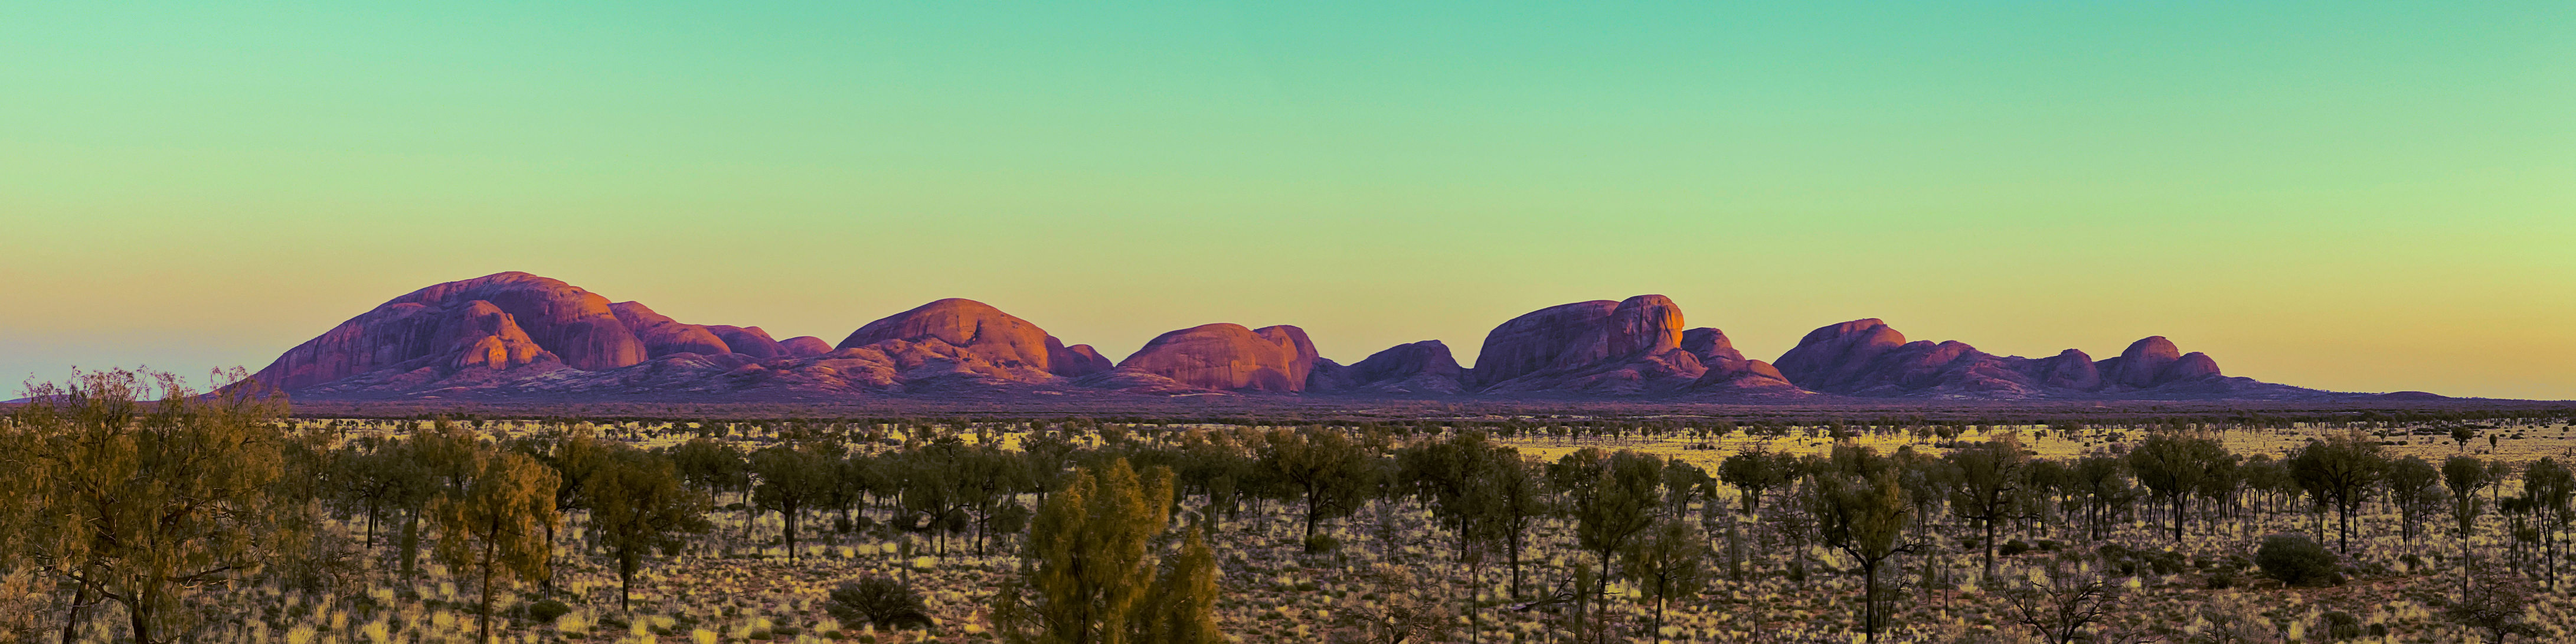
\includegraphics[width=1.0\textwidth]{kata-tjuta-morning.jpg}}
\caption{Kata Tjuta morning.}
\label{fig:7573x3}
\end{figure}

%\begin{figure}
%\centering
%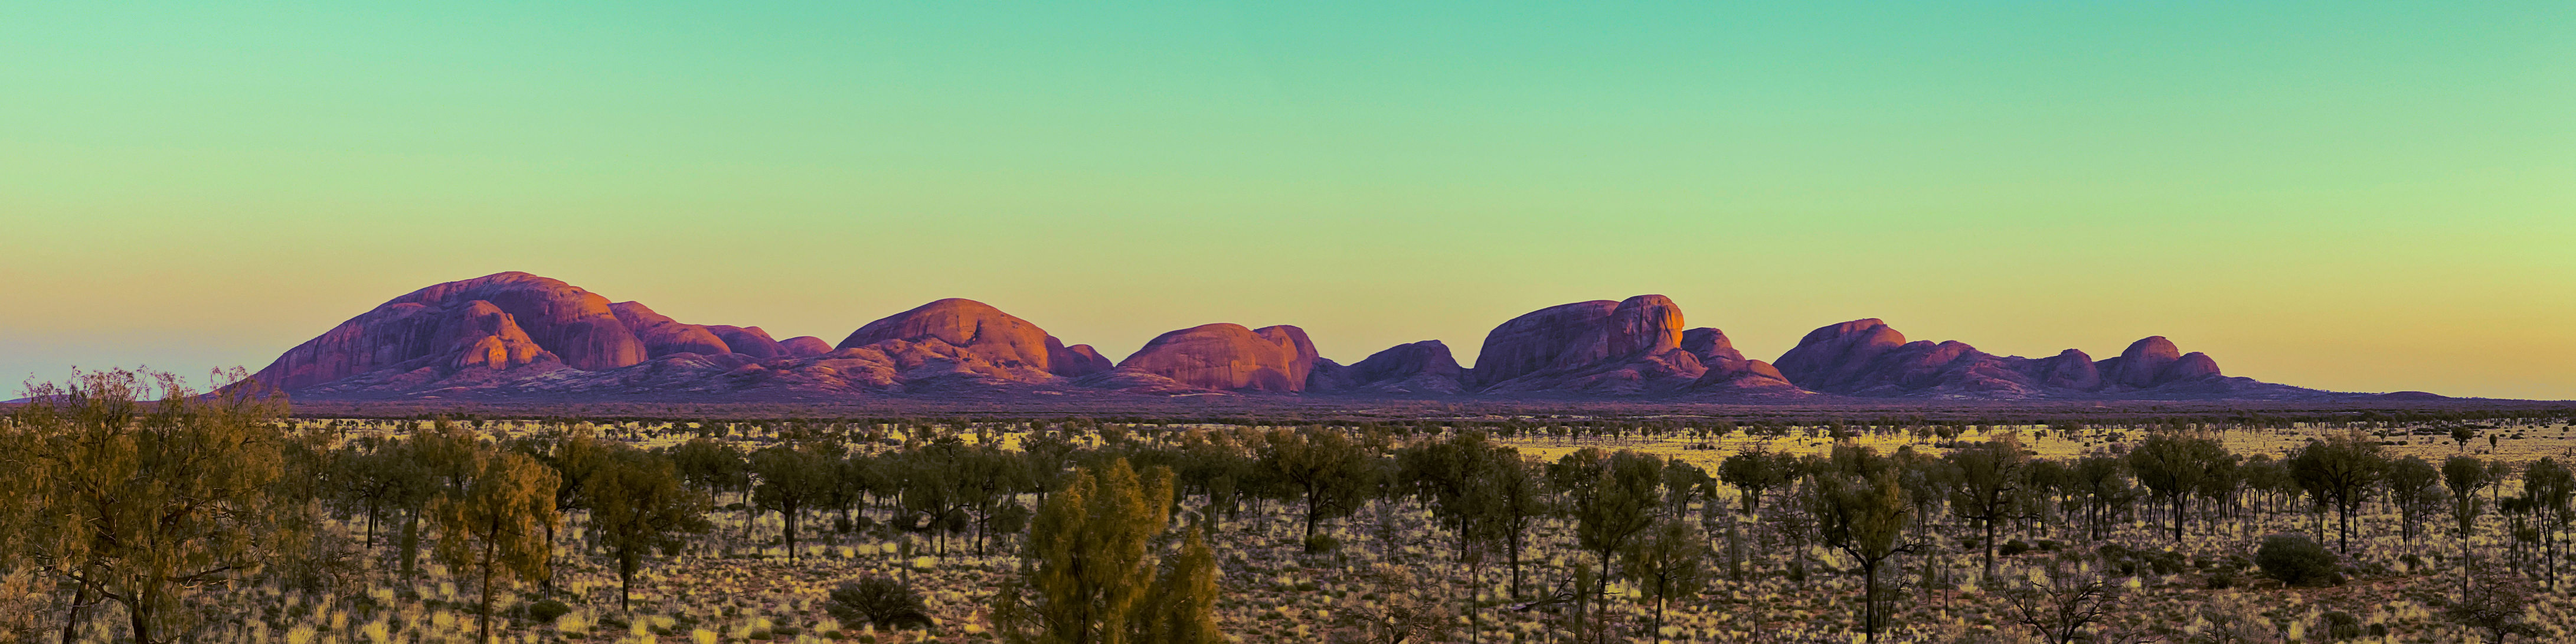
\includegraphics{kata-tjuta-morning.jpg}
%\caption{Kata Tjuta morning.}
%\end{figure}

After the hike, I caught the bus back to the Hotel and met Mali in the
hotel gardens. We had lunch and at 11:20 am took the ``Hop on Hop Off''
bus to Uluru. It was midday when we left the bus at the Mutitjulu
Waterhole trail so I screwed on my polarizing filter. The filter brought
out the red in the rocks. We saw the waterhole. It's a catch basin,
rainwater, gathered from the surface of Uluru, drains to the Mutitjulu
Waterhole. The pool is one of the few spots around Uluru where standing
water might be found year-round; it's considered sacred by the
Aborigines.

The Anangu people are now managing Uluru and they have marked many of
their sacred sites. As you walk around Uluru, you will see little signs
imploring you not to take pictures of certain areas. It's hard to
respect silly religious nonsense no matter what the religion. Aboriginal
beliefs are just as ridiculous as Islamic and Christian beliefs. Belief
remains a bullshit word but I mostly respected the signs regarding
photographs.

We kept walking around the base of Uluru until we reached the car park where
people once climbed the rock. Climbing is now banned. The Anangu never
approved of climbing and now that they are administering the rock,
they've banned it. I approve of the ban, not because of any sky fairy
sacred rock nonsense, but simply because it cuts down on the number of
yahoos. Without the ban, the parking lot would have been filled with
four-wheel drive trucks loaded with noisy tourists decked out in gay
Spiderman climbing suits. Instead, the lot was empty and we were the
only people beside this world wonder. As I have said over and over, I
prefer my national parks with fewer people.

At the car park, we cut across the plain beside Uluru to the aboriginal
cultural center where we ate some ice cream and looked at very nice and
very expensive aboriginal paintings. We then caught the bus back to the
Ayers Rock Resort and had dinner in the Ilkuri restaurant in the
\href{https://www.ayersrockresort.com.au/accommodation/sails-in-the-desert}{Sails
in the Desert Hotel}. Mali complained about the food as usual. Nothing
is cooked to her satisfaction. Even top-rated restaurants seldom match
her cooking. It's both a pleasure and a curse to be married to an
extreme foodie.

After dinner, we were scheduled for a family astronomy tour but Mali
decided to stay in our room. I went by myself. About three or four
families with young children attended. The session was held about 300
meters from the resort behind a small rise so the skies were not as dark
as the unexpected but stunning after-dinner star party by Uluru the
previous night. The Magellanic clouds were obscured by trees and resort
glow but the view to the south was great. As the tour guides delivered
their presentation I sat and watched the sky through my 8x42s. The
Butterfly Cluster was brilliant at this latitude. Cygnus was low and
inverted on the horizon. Vega, instead of being near the zenith, was
close to the horizon. The session included views through a
computer-driven 8-inch Celestron telescope. I mostly let the others
enjoy the sights but I did peek at Jupiter mostly to compare it with
what I see in my 245 mm DOB telescope. My DOB, from my backyard in
Meridian Idaho, shows Jupiter better.

It was a long day when I got back to our room. Mali was still awake
watching Bridesmaids on TV.

The next morning, we got up and packed for the flight to Sydney. I don't
like constantly packing and unpacking. Flying is worse because of
carry-on and luggage restrictions. I have two camera bags. Two bags
technically exceed the carry-on count so I tie the two bags together
with shoelaces and Velcro to turn two easily carried camera bags into
one shoulder-crushing bag. I have tied and untied my bags many times.
It's annoying.

Our Jetstar flight 661 from Ayers Rock Airport to Sydney was on time and
because the airport was small the usual hellish modern airport
experience was minimized. On take-off, the plane was hit by a strong
side gust of wind that pushed it sideways just as the wheels left the
ground. This freaked out Mali. She clung to me and said she wanted off
and that the pilot didn't know what he was doing. She's been a nervous
flyer ever since a bad bit of turbulence on a flight to Calgary Canada
in 2006.

We made it to Sydney. The landing was pretty smooth. At the airport, we
caught the train to downtown Sydney. You can board Sydney trains by
simply tapping on and off with a credit card. This makes so much sense
that I'm surprised it hasn't spread to all civilized countries. It
wouldn't work in the US but it's hard to consider the US civilized these
days.

We exited the train at Wynyard station and dragged our luggage through
city streets to the hotel. When we checked the VISA charges later it was
89 Canadian cents to ride from the airport: easily the biggest bargain
so far. Mali was proud of herself for insisting we take the train. Today
we are boarding the cruise ship for our 12-day circumnavigation of New
Zealand. I think I will enjoy being in a hotel that moves and not having
to pack and unpack for a while.


\captionsetup[figure]{labelformat=empty}
\begin{SCfigure}[50]
\centering
\href{https://conceptcontrol.smugmug.com/Trips/Overseas/Australia-New-Zealand-2022/i-W97WzvW/A}{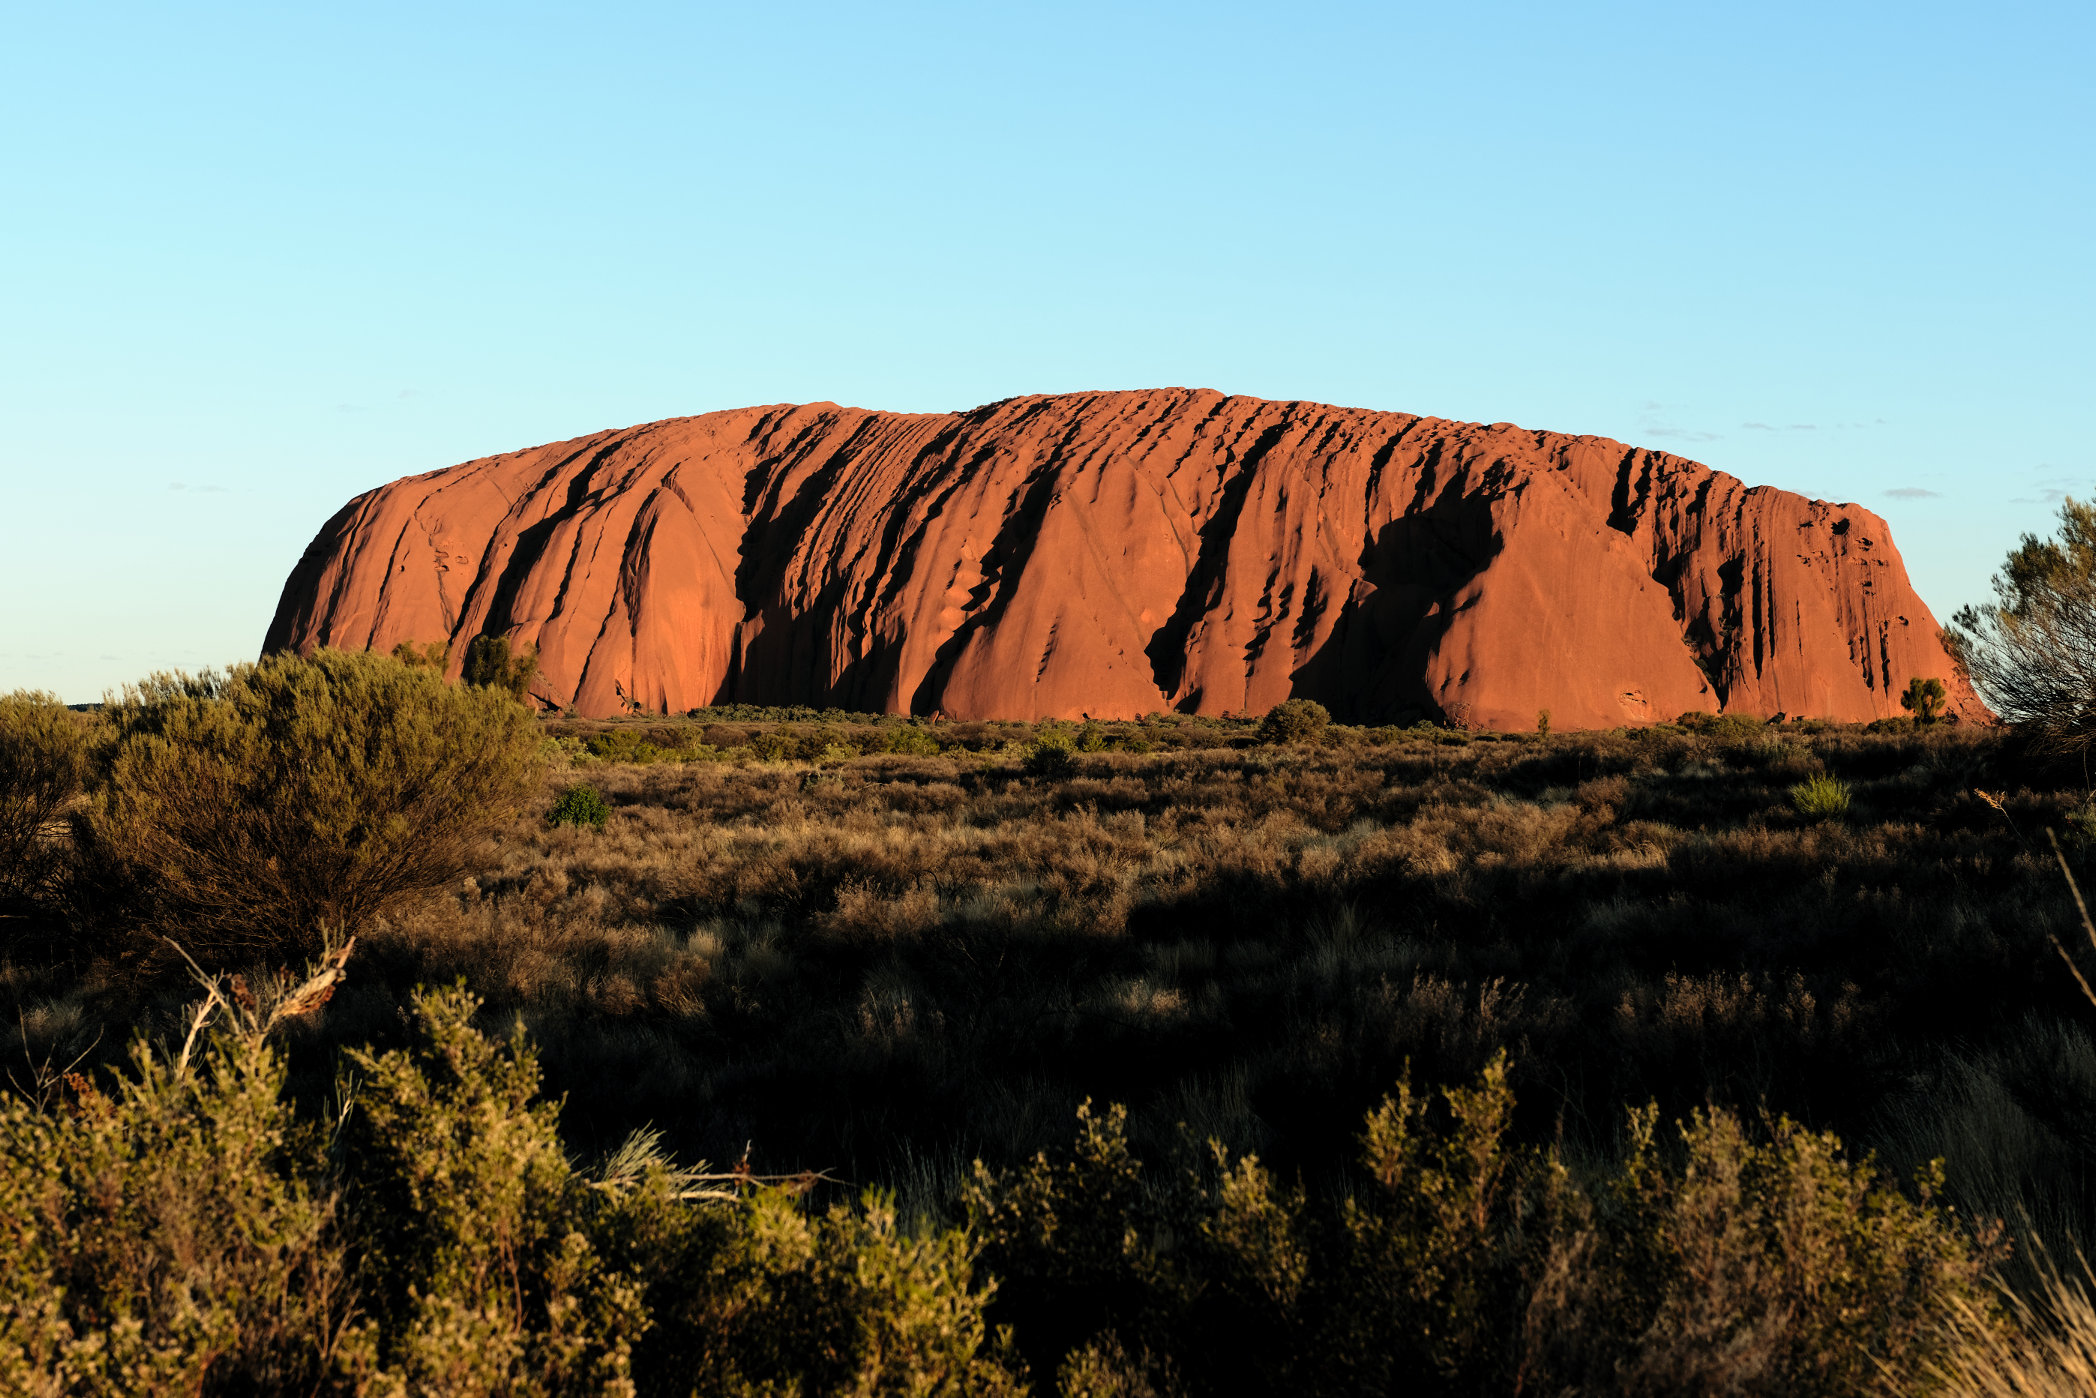
\includegraphics[width=0.40\textwidth]{uluru-wet-spring.jpg}}
\caption[Uluru in spring]{The wetter-than-usual Australian spring extended into the
interior of the continent. Our bus driver said that the vegetation
around Uluru was about as lush as it ever gets. Lucky me, foreground
vegetation contrasts nicely with the stunning reds of Uluru.}
\label{fig:7573x4}
\end{SCfigure}

%\end{document}

